\chapter{头痛和面痛}

头痛(headache)是指位于眼眶耳孔基线以上的疼痛;面痛(facial
pain)则是指位于眼眶耳孔基线以下、脖子以上和耳朵以前的疼痛。

\section{【头痛疾病的分类】}

分类见表\ref{tab46-1}

\begin{longtable}{c}
 \caption{头痛疾病的分类}
 \label{tab46-1}
 \endfirsthead
 \caption[]{头痛疾病的分类}
 \endhead
 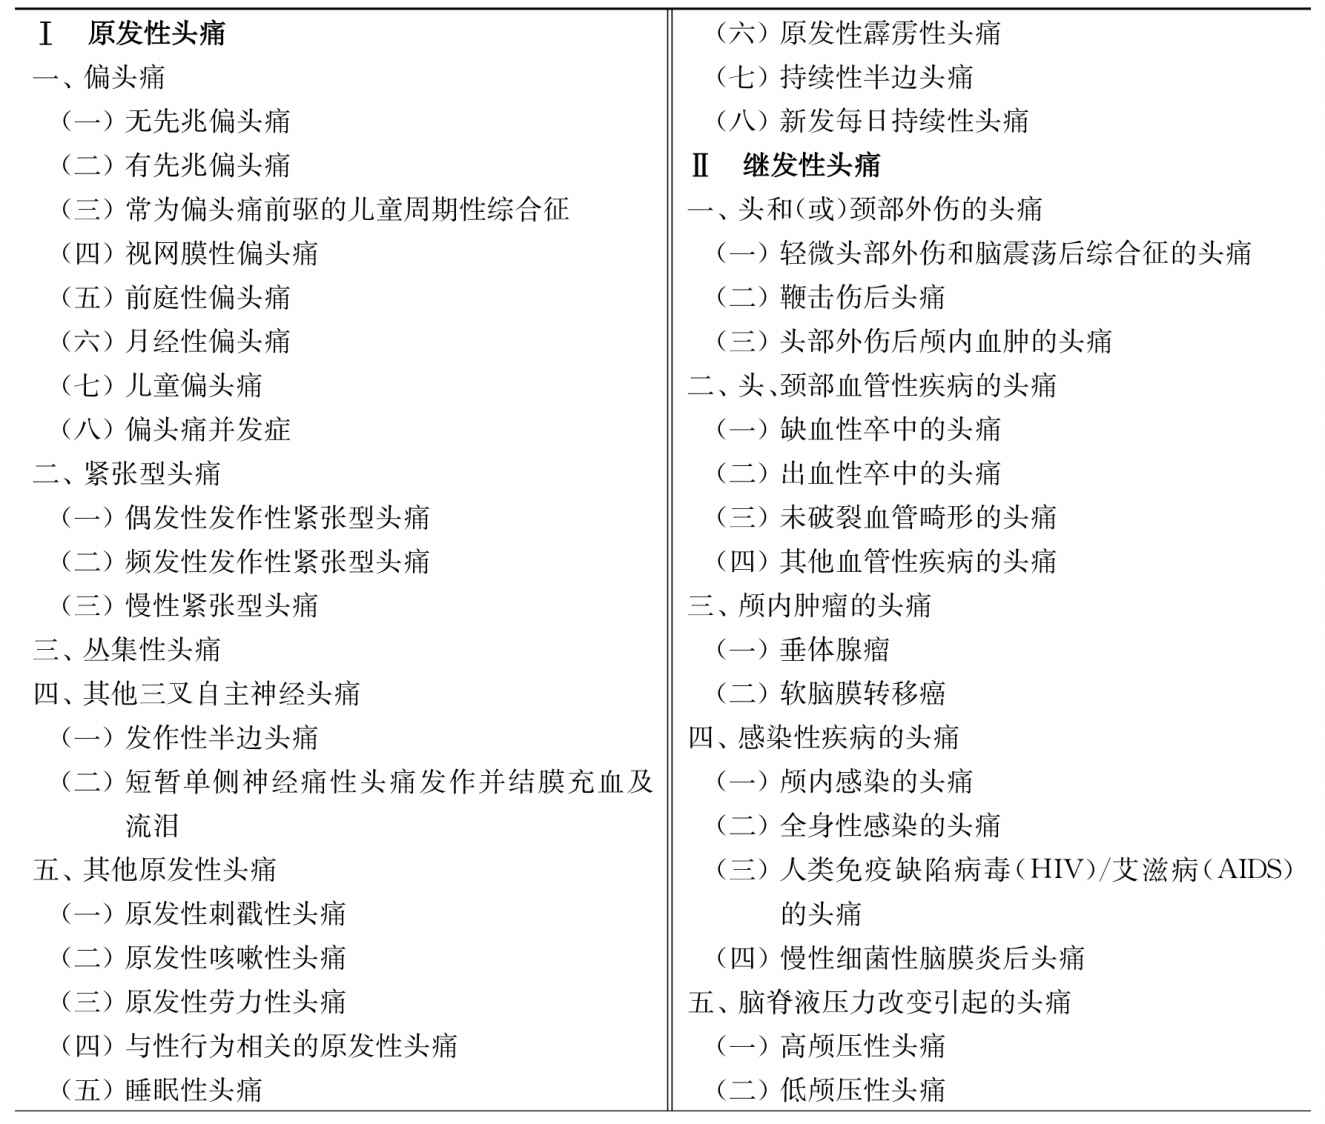
\includegraphics[width=\textwidth,height=\textheight,keepaspectratio]{./images/Image00275.jpg}\\
 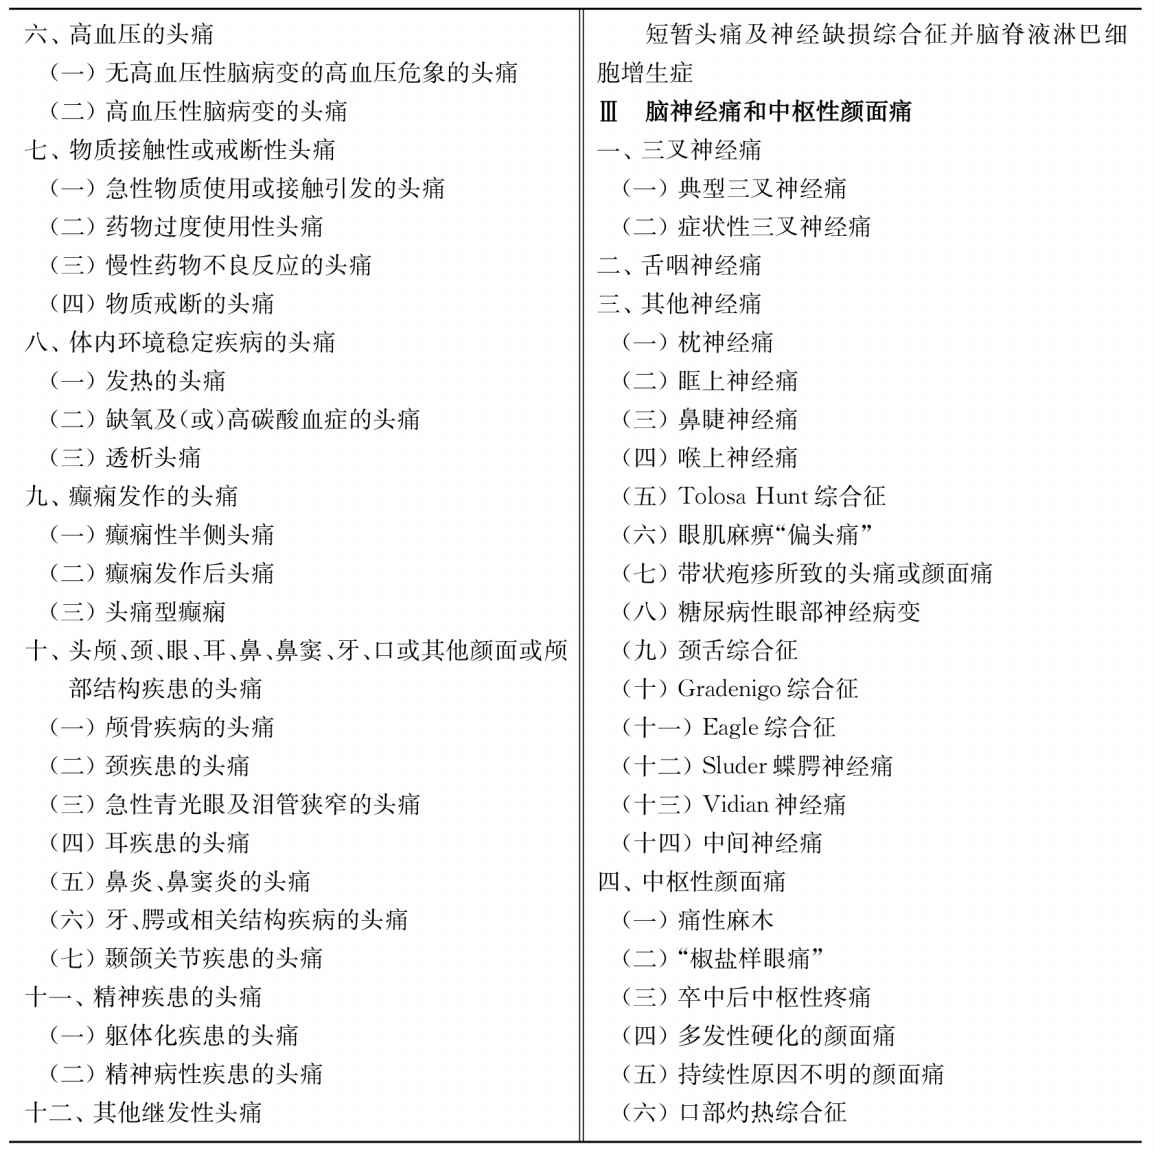
\includegraphics[width=\textwidth,height=\textheight,keepaspectratio]{./images/Image00276.jpg}
 \end{longtable}

\section{【头痛发生的机制】}

头痛可由于下列组织的病变引起:①血管改变:血管被伸展、移动、挤压,如脑肿瘤、脑水肿、脑出血;颅内、外动脉高度扩张,血流冲击松弛的血管壁,刺激痛觉神经末梢或使血管壁发生震动而致头痛,见于偏头痛、发热、低氧、低血糖、一氧化碳中毒、使用扩张血管药、癫痫大发作后;颅内静脉扩张,牵引痛敏结构发生头痛,见于肺气肿、心功能不全、腰穿后;血管炎症,如颞动脉炎、静脉窦炎、各类脉管炎;颅内小血管收缩或痉挛,如蛛网膜下腔出血时,血浆中的游离肽和血小板破坏后释放出的5-羟色胺均可刺激颅内小血管收缩或痉挛,产生头痛。②脑膜病变:脑膜炎、脑水肿、蛛网膜下腔出血、脑膜癌病等皆可刺激或牵引脑膜而产生头痛。③肌肉病变:额、颞、枕、颈后、头顶和肩背诸肌可由于各种病变发生收缩,导致头痛,称为“紧张型头痛合并颅周压痛”(旧称肌收缩性头痛)。④神经病变:含有痛觉纤维的神经由于本身或邻近组织的病变而发生激惹、挤压、绞榨、牵引等引起面痛,如三叉神经痛。⑤五官和颈椎病变:可直接刺激、牵引或压迫邻近的痛敏结构,引起头痛和颅面痛。⑥生化改变:如偏头痛的发生与5-羟色胺、降钙素基因相关肽等的改变密切相关。⑦内分泌改变:绝经期头痛、月经期头痛、偏头痛等均与内分泌有关。⑧其他:遗传因素、食物因素、过敏。

总之,头痛的发生机制异常复杂,有些头痛并非单一因素构成,而是上述多种机制复合所致。

\section{【头痛病因鉴别的相关检查】}

详尽的病史和神经系统尤其是眼底检查的重要性自不待言,其他系统特别是血压、血脂、血糖、五官、颈椎等的检查非常重要,辅助检查应在病史以及体检的基础上选择相应的项目进行,如神经影像学、电生理、脑脊液、脑磁图、CT+PET、MRI+PET、SPECT、DSA等。

\section{【头痛鉴别诊断的思路】}

\subsection{(一)性别及年龄}

偏头痛女性患者4倍于男性;丛集性头痛男性患者3倍于女性;发作性半侧头痛患者大部分为女性;巨细胞动脉炎多发生于60岁以上的患者;颅面神经痛多发生于成年以后,少见于儿童和青少年。

\subsection{(二)头痛部位}

尽可能弄清楚头痛的部位是单侧或双侧、前头或后头、局部或弥漫、表浅或深在。颅外病变其头痛多较局限及表浅,常在刺激点附近或神经分布区内;颅内病变其头痛多较弥散及深在。小脑幕以上病变的疼痛一般位于额、颞和顶区;小脑幕以下者一般位于耳后、枕、颈上部,也可放射至前额。半侧头痛是偏头痛、发作性半侧头痛的特点。弥漫性全头痛常见于颅内感染、颅脑外伤、颅内高压、脑出血。枕颈部痛见于枕神经痛、颈源性头痛、蛛网膜下腔出血。半侧面痛见于三叉神经痛、带状疱疹后神经痛等。

\subsection{(三)头痛性质}

搏动性痛是偏头痛的特征,也是诊断偏头痛的标准之一;紧缩感、压迫感、钳夹样痛是紧张型头痛的特点;霹雳性头痛(thunderclap
headache)见于蛛网膜下腔出血;尖锐、电击样痛是颜面神经痛的特征。

\subsection{(四)头痛程度}

大致分为轻、中、重度,但与疾病的轻重不一定呈正相关,一般以霹雳性头痛、脑膜刺激性头痛、偏头痛、三叉神经痛最剧。妨碍患者入睡或使患者痛醒的头痛,常有器质性疾病的基础。

\subsection{(五)头痛发生的方式及经过}

必须注意头痛是急性、亚急性抑或慢性发生。其过程为波动性、持续进展、周期发作抑或慢性复发性。急起尤其是第一次出现的剧烈头痛更需警惕,因其病因多属器质性。头痛呈周期性发作是偏头痛的特征;持续进展见于颅内占位性疾病;亚急性进展见于硬膜下血肿、脑脓肿;慢性头痛见于颅内占位性疾病、慢性紧张型头痛。

\subsection{(六)头痛出现的时间与持续时间}

某些头痛发生在特定的时间,如清晨、日间、入睡后、月经前或月经期间。丛集性头痛常在夜间入睡后发作;三叉神经痛多在日间发生;头痛的持续时间则有数秒、数分钟、数日、数月甚至数年不定。典型三叉神经痛和舌咽神经痛发作时疼痛往往持续数秒至几十秒;紧张型头痛则常经年累月,其间有波动性。

\subsection{(七)加重、减轻或激发头痛的因素}

咳嗽、打喷嚏、大笑、摇头、俯首以及弯身等动作可促使颅内高压性头痛、偏头痛、颅内感染性头痛、脑肿瘤等的头痛加剧(用力性头痛的特点)。偏头痛的诊断标准之一是“日常体力活动如走楼梯可加重头痛”;颅内低压性头痛可因卧床减轻或消失,而直立位则头痛出现或加重,也可因注射低渗溶液而减轻;高颅压头痛则需注射高渗溶液才能缓解;丛集性头痛取直立位可减轻;压迫颞动脉或颈总动脉可减轻由于颅外动脉扩张而引起的头痛。使用一些药物可产生头痛,但突然撤停某些长期服用的药物如麦角胺,可发生“撤停性头痛”。碰触患侧面部的扳机点可诱发典型的三叉神经痛,发作性半侧头痛服用治疗量的吲哚美辛往往可完全预防发作。

\subsection{(八)伴随症状与体征}

特别注意患者有无发热、眩晕、恶心、呕吐、发作性或持续性视力减退、视野缺损、眼肌瘫痪、瞳孔改变、眼底改变、鼻腔、鼻窦、耳部、口腔、牙齿、咽喉症状;精神症状;意识障碍;脑膜刺激征;抽搐;肢体麻木或瘫痪;共济失调;血压等。如急性颅内感染性头痛时,发热与头痛同时发生或发热先于头痛出现;颅内高压症的头痛常伴有头晕或眩晕;发作性视力减退、视野缺损是有先兆偏头痛(migraine
with
aura)的常见先兆。单侧眼及眼周痛伴有3、4、6对脑神经瘫痪(完全或不完全)很有可能是Tolosa
Hunt综合征,但如伴有眼球突出、发热则要考虑有否海绵窦血栓性静脉炎,偶尔也可见于海绵窦内的颈内动脉瘤扩张,压迫周围的3、4、6对脑神经所致。头痛发作时伴有流泪、流涕、眼及(或)该侧面部充血等,见于三叉神经痛。此处提出一组“伴有局灶性神经症状或体征的头痛”的疾病或综合征,其鉴别诊断较为复杂。属于这类头痛的疾病或综合征有下列16种:有先兆偏头痛;眼肌瘫痪型偏头痛;丛集性头痛和其他三叉自主神经痛;缺血性卒中和短暂性脑缺血发作;脑出血;蛛网膜下腔出血;未破裂的血管畸形;动脉炎;颈动脉或椎动脉疼痛;大脑静脉血栓形成;高脑脊液压力;低脑脊液压力;脑肿瘤;短暂性头痛和神经功能缺失伴脑脊液淋巴细胞增生综合征(HaNDL);三叉神经痛(痛性抽搐);Tolosa
Hunt综合征;急性带状疱疹和带状疱疹后神经痛。这些疾病所引起的头痛的特点见本章有关内容。

对头痛的鉴别首先要区分是原发性还是继发性。前者基本上是良性疾病,而后者主要是脑部结构损害所致。在发作性头痛中,如神经症状或体征在头痛之前,则很可能为原发性头痛;如神经症状或体征伴随头痛发生或持续存在,则极可能为症状性头痛(继发性头痛)。超过数周或数月的头痛并伴有局灶性神经症状或体征,肯定是继发性头痛,参考图\ref{fig46-1}。

\begin{figure}[!htbp]
 \centering
 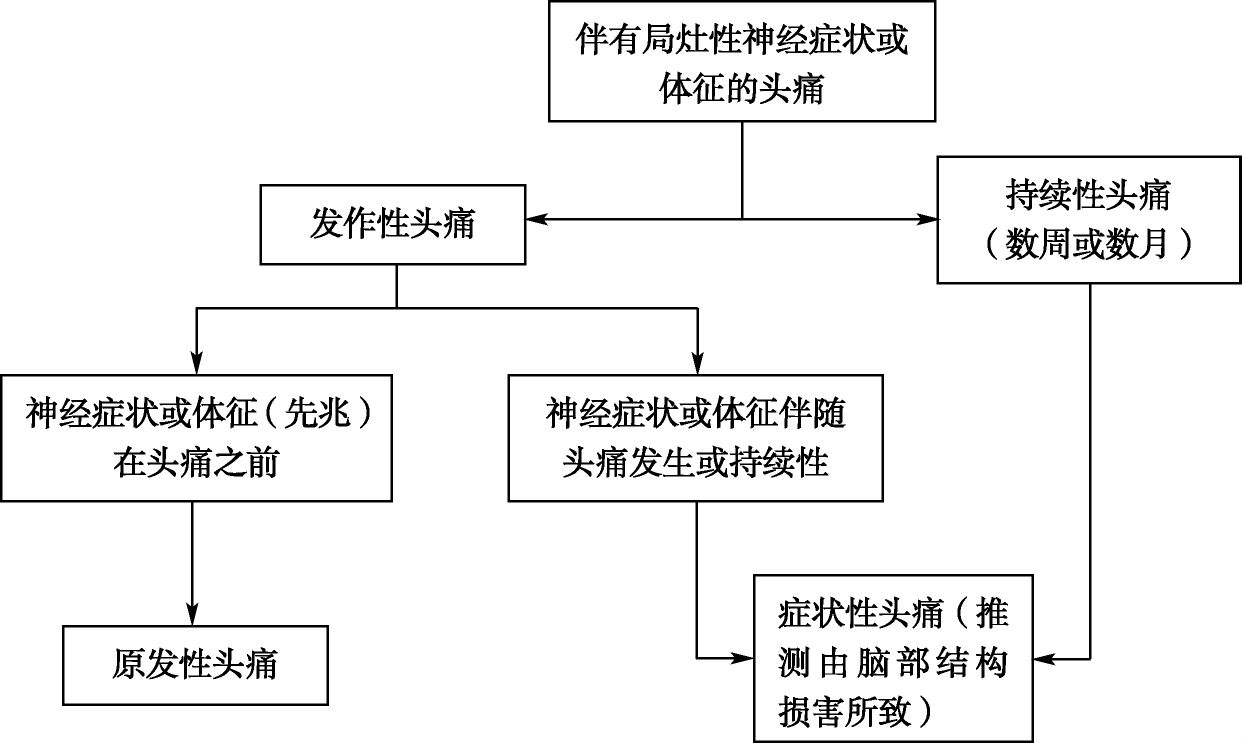
\includegraphics[width=4.34375in,height=2.5625in]{./images/Image00277.jpg}
 \captionsetup{justification=centering}
 \caption{伴有局灶性神经症状或体征的头痛的鉴别诊断}
 \label{fig46-1}
  \end{figure} 

\protect\hypertarget{text00347.html}{}{}

\section{154 原发性头痛}

\subsection{一、偏头痛}

偏头痛(migraine)是一种反复或周期性发作、表现为单侧或双侧搏动性头痛的疾病,头痛持续数分钟至数天,常伴恶心、呕吐,可有或无先兆。世界卫生组织对全球所有会造成失能的疾病进行排列,偏头痛位列第19位,并将严重偏头痛与痴呆、四肢瘫痪和严重精神病一起定为最致残的慢性疾病,可见本病对人类所造成的巨大灾害。此外,偏头痛除疾病本身可造成损害外,还可以进一步导致其他损害。偏头痛是脑卒中的一项独立危险因素,偏头痛的反复发作还可导致脑白质病变、认知功能减退,偏头痛可与多种疾病共患,如癫痫、抑郁症及情感性精神障碍等。偏头痛的患病率在全球为10\%~12\%;美国12.6\%;亚洲平均8\%;中国平均7\%(2001年)。偏头痛多在青春期发病,好发年龄为25~35岁,男女患者比例为1∶4。

已知有许多因素可引起或加重偏头痛的急性发作:①食物与饮食习惯:包括奶酪、巧克力、牛奶和其他奶制品、亚硝酸盐、咖啡、动物脂肪等;②气候和季节变化:偏头痛在春夏季多发,尤其是湿热的气候条件;③精神心理因素:不良情绪、压力、睡眠障碍、疲劳等精神心理因素与头痛的发作关系密切且相互影响、互为因果;④吸烟与饮酒:吸烟包括被动吸烟可诱发1\%~61\%的患者发生头痛,乙醇尤其是红酒是头痛可能的主要诱发因素之一;⑤感官刺激:光线、噪音、气味可能诱使偏头痛发作;⑥药物作用:口服避孕药、硝酸甘油、西洛他唑、利血平、肼苯达嗪、雷尼替丁、西地那非等可诱发偏头痛发作;⑦其他相关诱发因素:包括头部创伤、性生活、月经来潮、癫痫发作和从事强体力活动等。

关于偏头痛的发生,目前三叉神经血管反射学说被认为是偏头痛发病机制的主流学说,以5-羟色胺(5-hydroxytryptamine,5-HT)、降钙素基因相关肽(calcitonin
gene-related peptide,CGRP)和P物质(substance
P,SP)为代表的血管活性物质在偏头痛发病过程中发挥着至关重要的作用。

三叉神经血管反射学说:Moskowitz发现三叉神经血管系统或中枢神经内源性疼痛调节系统存在功能缺陷,分布于硬脑膜的三叉神经无髓C纤维受到刺激时,释放血管活性物质如CGRP、SP、神经激肽A等,产生神经源性炎症,使血管扩张、血浆成分外渗、肥大细胞脱颗粒和血小板激活,提出了三叉神经血管反射学说,是目前研究偏头痛发病机制的主流学说,它将神经、血管、递质三者相结合,主要涉及三种机制:供应脑膜的颅内脑外血管扩张、血管周围神经释放血管活性肽引起神经源性炎症以及中枢痛觉传导的抑制性降低。

在血管舒缩过程中,5-HT是受体和靶细胞间的介导物,其代谢紊乱是偏头痛发病的物质基础,在偏头痛的先兆期、发作期等不同时相介导不同的病理过程。临床上很多治疗偏头痛的药物如曲坦类是通过作用于5-HT递质或受体预防和改善偏头痛发作的。CGRP是由37个氨基酸组成的生物活性多肽,是迄今已知的最强大的血管舒张肽,是三叉神经微血管激活的标志物,在疼痛感觉和调控中发挥着重要的作用。Cady等发现CGRP可以促进三叉神经元与神经胶质细胞在中枢和外周的敏感性。在偏头痛发作期间,CGRP水平明显增高。SP是速激肽家族中的一种11肽,是传递并降低痛阈值的神经递质,另外,SP的前体为前速激肽原,致血管扩张作用仅次于CGRP。

其他与偏头痛发生有关的因素包括:①TXA\textsubscript{2}
和PGI\textsubscript{2}
平衡障碍;②血小板功能异常;③内分泌改变:偏头痛最常始于青春期,多在更年期后渐减轻或消失,生育期的女患者大约有60\%在妊娠期偏头痛停止发作,分娩后可复发,提示偏头痛的发生与内分泌有关;④遗传因素:偏头痛一向被认为是多基因遗传病,近年发现家族性偏瘫性偏头痛(familial
hemiplegic migraine,FHM)则为单基因遗传病。

偏头痛的临床表现:偏头痛发作可分为前驱期、先兆期、头痛期和恢复期,但并非所有患者或所有发作均具有上述四期。同一患者可有不同类型的偏头痛发作。

\subsubsection{1.前驱期}

头痛发作前,患者可有激惹、疲乏、活动少、食欲改变、反复哈欠及颈部发硬等不适症状,但常被患者忽略,应仔细询问。

\subsubsection{2.先兆期}

先兆指头痛发作之前出现的可逆的局灶性脑功能异常症状,可为视觉性、感觉性或语言性。视觉先兆最常见,典型的表现为闪光性暗点,如注视点附近出现“之”字形闪光,并逐渐向周边扩展,随后出现“锯齿形”暗点。有些患者可能仅有暗点,而无闪光。其次是感觉先兆,表现为以面部和上肢为主的针刺感、麻木感或蚁行感。先兆也可表现为言语障碍,但不常发生。先兆通常持续5~30分钟,不超过60分钟。

\subsubsection{3.头痛期}

约60\%的头痛发作以单侧为主,可左右交替发生,约40\%为双侧头痛。头痛多位于颞部,也可位于前额、枕部或枕下部。偏头痛的头痛有一定的特征,程度多为中至重度,性质多样但以搏动性最具特点。头痛常影响患者的生活和工作,行走、登楼、咳嗽或打喷嚏等简单活动均可加重头痛,故患者多喜卧床休息。偏头痛发作时,常伴有食欲下降,约2/3的患者伴有恶心,重者呕吐。头痛发作时尚可伴有感知觉增强,表现为对光线、声音和气味敏感,喜欢黑暗、安静的环境。其他较为少见的表现有头晕、直立性低血压、易怒、言语表达困难、记忆力下降、注意力不集中等。部分患者在发作期会出现由正常的非致痛性刺激所产生的疼痛(allodynia)。

\subsubsection{4.恢复期}

头痛在持续4~72小时的发作后可自行缓解,但患者还可有疲乏、筋疲力尽、易怒、不安、注意力不集中、头皮触痛、欣快、抑郁或其他不适。

根据国际头痛协会2004年制定的第二版“头痛疾患的国际分类”(ICHD-Ⅱ),将偏头痛分为6个亚型:

\subsubsection{(一)无先兆偏头痛(migraine without aura,MO)}

也称普通偏头痛,是临床最常见类型,约占偏头痛患者的80\%,鲜有家族史。MO系指无明确先兆症状(如视觉先兆、感觉先兆和语言先兆)的发作性偏头痛,它是一种反复发作的头痛,典型特征为单侧、额颞部、搏动性头痛,发作持续4~72小时,程度中或重度,日常活动会加剧头痛,常伴恶心、呕吐和(或)畏光、畏声(表\ref{tab46-2})。本型偏头痛在女性患者与月经关系密切。

\begin{table}[htbp]
\centering
\caption{无先兆偏头痛的诊断标准}
\label{tab46-2}
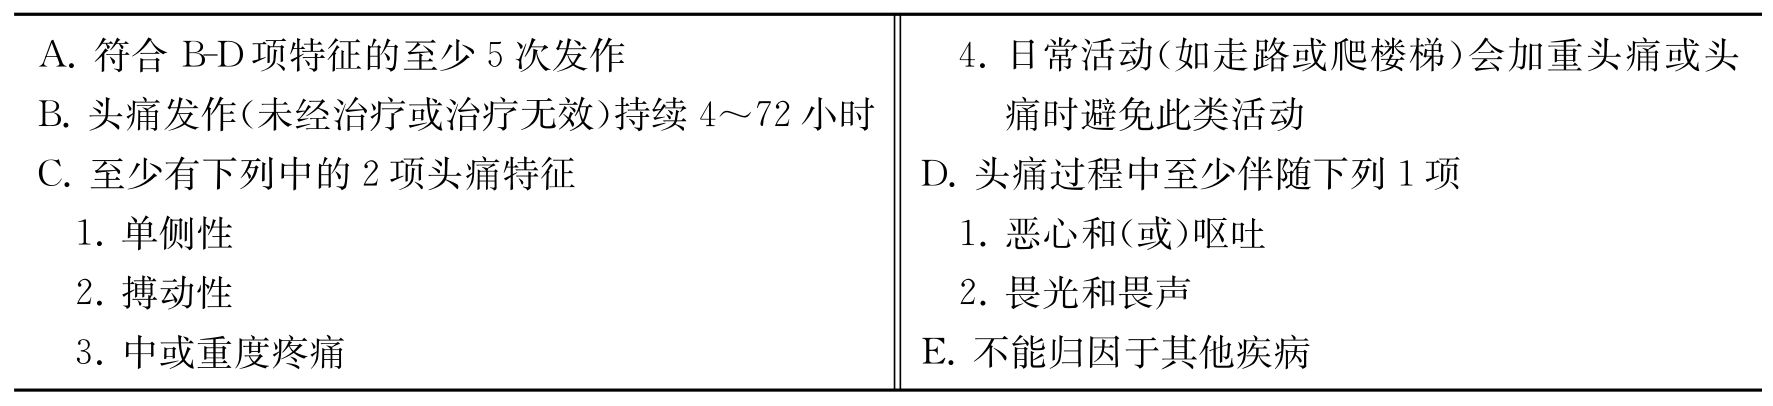
\includegraphics[width=5.90625in,height=1.34375in]{./images/Image00278.jpg}
\end{table}

\subsubsection{(二)有先兆偏头痛(migraine with aura,MA)}

旧称典型偏头痛,占全部偏头痛的15\%~18\%,此型具有遗传特征,60\%~80\%的病例在同一家庭的同代人或连续几代人中发生。MA的先兆是指在头痛发作前出现短暂的局灶性神经症状,通常在5~20分钟内逐渐发生,持续不超过60分钟;头痛具备上述无先兆偏头痛的特征,常在先兆症状之后出现。少数情况下后继的头痛没有偏头痛的特征,甚至完全没有头痛(对这种情况的诊断较困难)。

有先兆偏头痛发作的5个阶段表现:①前驱期:发作前1天或发作当天情绪改变、面色苍白、打呵欠、食欲改变、恶心、颈部僵硬、肌肉疼痛、对光及声敏感等;②先兆期:先兆表现为自发性反复发作的视觉症状,如闪光、线条(典型者如城垛状)、暗点、视野缺失,或躯体感觉异常如针刺感、麻木等神经系统症状,常于5~20分钟发展到高峰,持续时间一般不超过60分钟;③发作期:中至重度头痛,被迫休息,甚至卧床睡觉,被迫服用止痛药;④缓解期:服止痛药或睡眠后头痛缓解;⑤后遗症期:头痛缓解后数天之内疲乏无力、烦躁、情绪不佳、尿频。

有先兆偏头痛共分六个亚型,其诊断主要根据先兆特征,需要有2次以上的先兆发作并排除继发性头痛的可能。

\paragraph{1.伴典型先兆的偏头痛性头痛}

如果典型先兆后1小时内出现偏头痛性头痛发作,即可诊断为伴典型先兆的偏头痛性头痛(表\ref{tab46-3})。对先兆及其他有类似表现的疾病(如短暂性脑缺血发作、癫痫)要慎重鉴别(表\ref{tab46-4}),特别是40岁以上才出现先兆,以负向特征(如偏盲)为主,或先兆时间延长或非常短,则应先排除其他病因。

\begin{table}[htbp]
\centering
\caption{伴典型先兆的偏头痛性头痛的诊断标准}
\label{tab46-3}
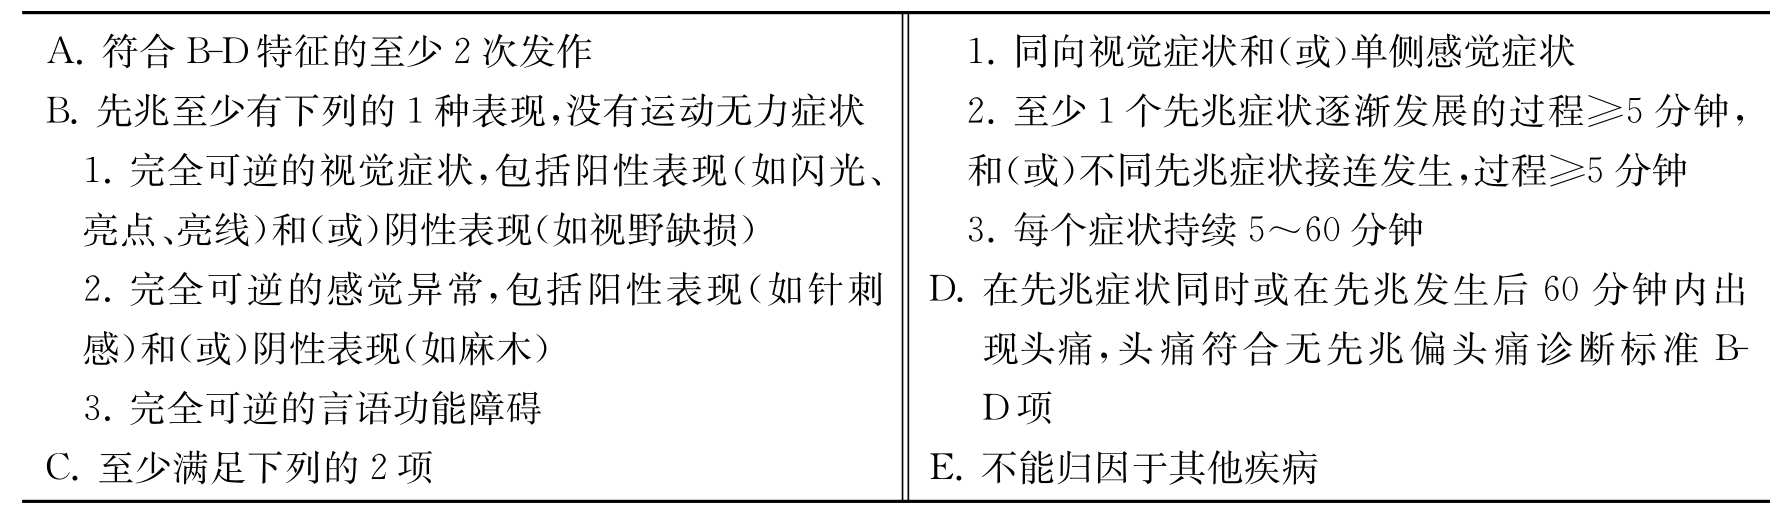
\includegraphics[width=5.9375in,height=1.70833in]{./images/Image00279.jpg}
\end{table}

\begin{table}[htbp]
\centering
\caption{局灶性发作性神经症状在三种疾病的鉴别诊断}
\label{tab46-4}
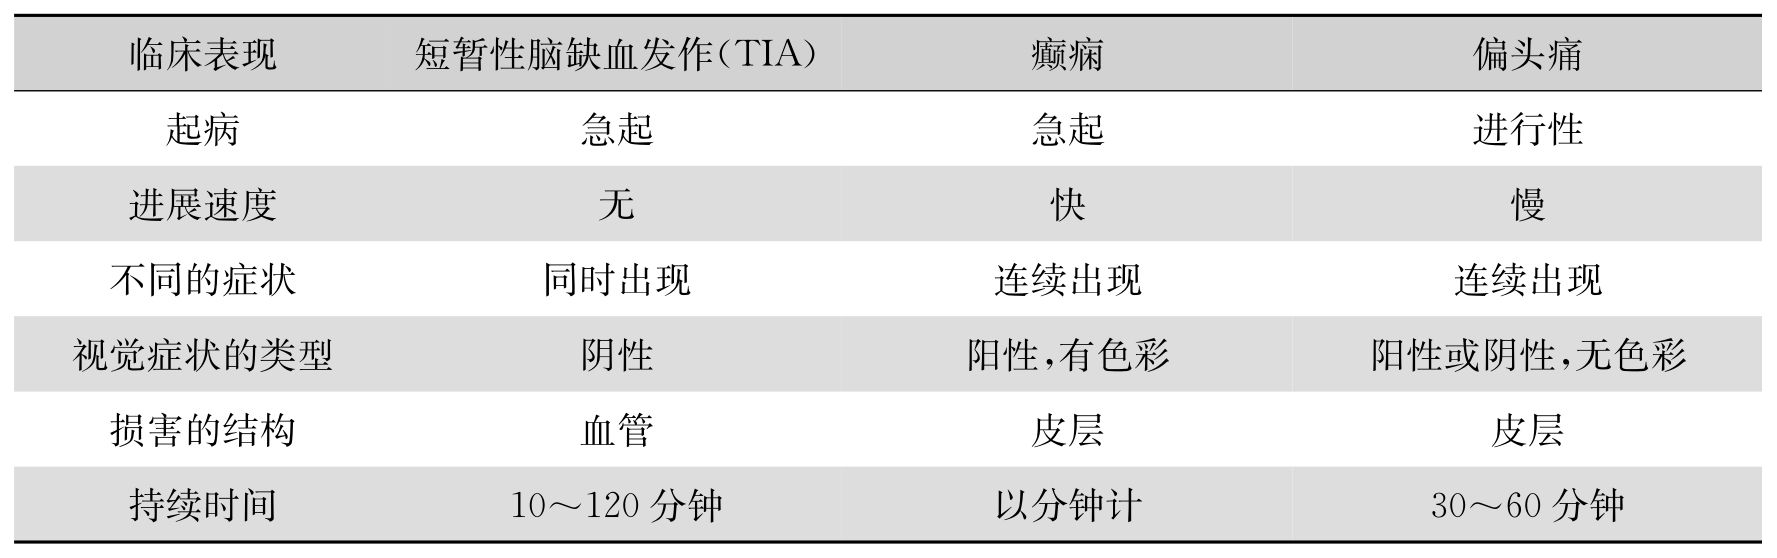
\includegraphics[width=5.91667in,height=1.85417in]{./images/Image00280.jpg}
\end{table}

\paragraph{2.伴典型先兆的非偏头痛性头痛}

如果典型先兆后的头痛不符合偏头痛性头痛的特点,则诊断为伴典型先兆的非偏头痛性头痛(表\ref{tab46-5})。

\begin{table}[htbp]
\centering
\caption{伴典型先兆的非偏头痛性头痛的诊断标准}
\label{tab46-5}
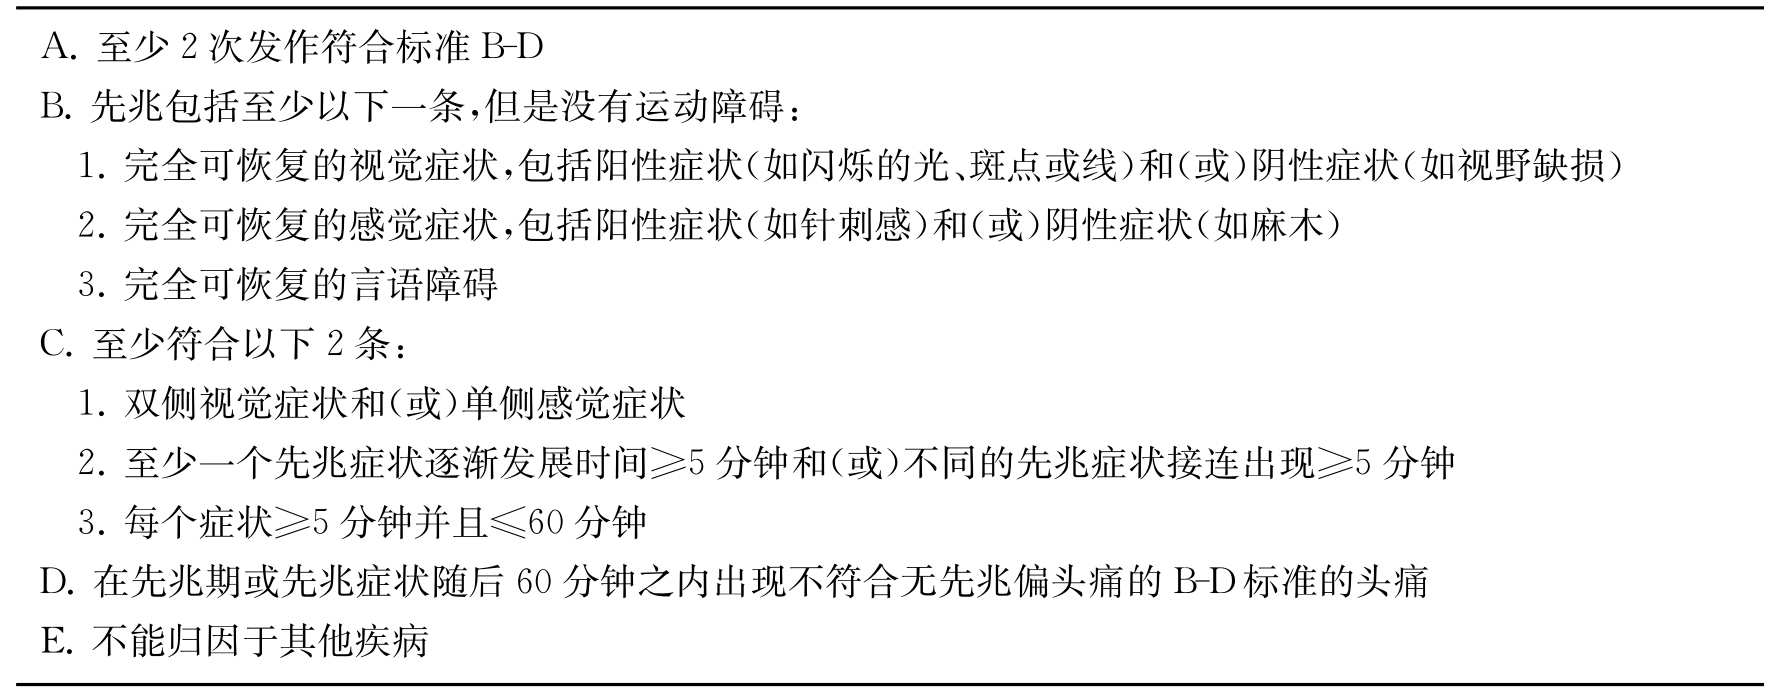
\includegraphics[width=5.91667in,height=2.32292in]{./images/Image00281.jpg}
\end{table}

\paragraph{3.典型先兆不伴头痛}

典型先兆后也可以没有头痛发作,此时诊断为典型先兆不伴头痛(表\ref{tab46-6})。

\begin{table}[htbp]
\centering
\caption{典型先兆不伴头痛的诊断标准}
\label{tab46-6}
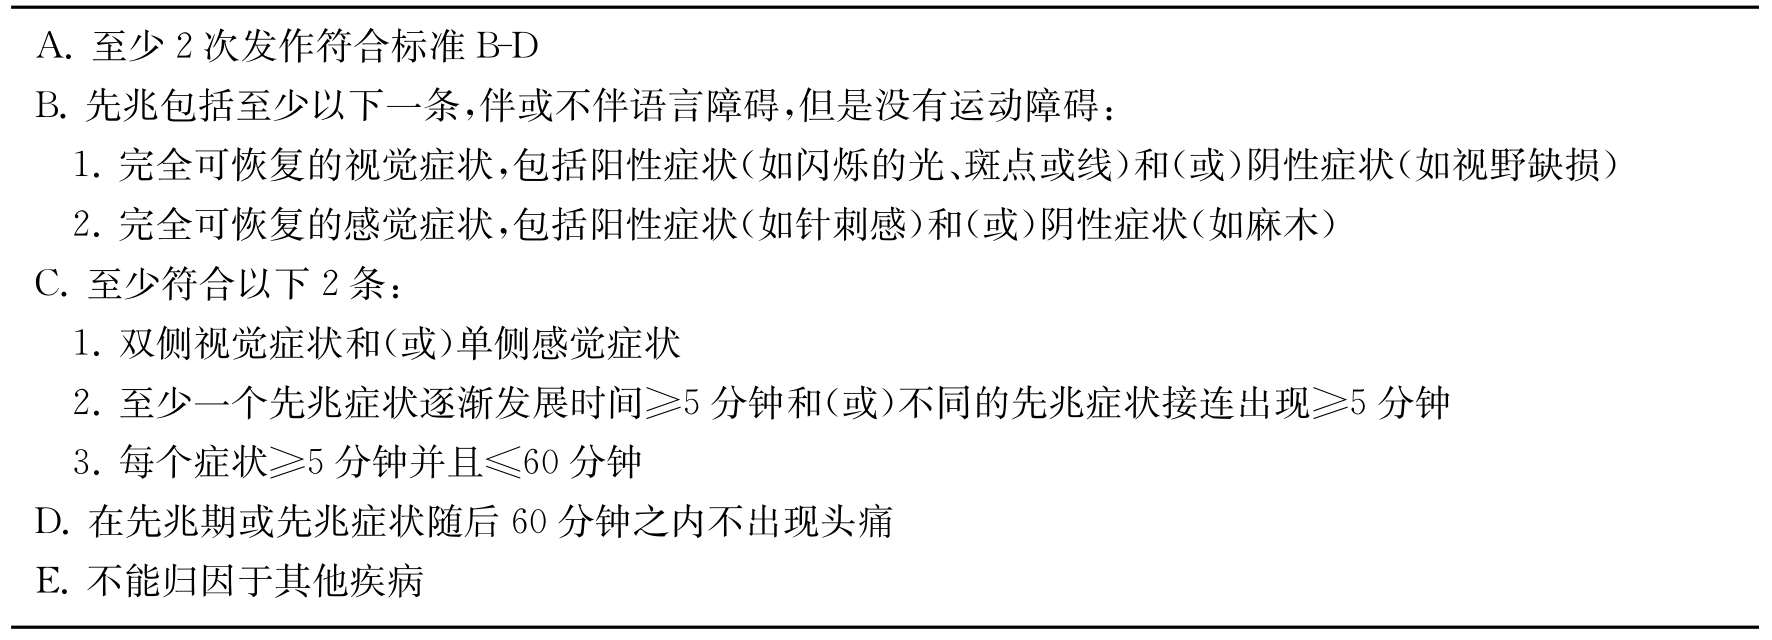
\includegraphics[width=5.89583in,height=2.125in]{./images/Image00282.jpg}
\end{table}

\paragraph{4.家族性偏瘫性偏头痛(familial hemiplegic migraine,FHM)}

一旦先兆期出现肢体无力表现,需考虑偏瘫性偏头痛,若患者的一、二级亲属中有类似发作,则诊断为家族性偏瘫性偏头痛(表\ref{tab46-7})。FHM按其基因突变分为FHM1和FHM2,前者的突变在19q的CACNA1A,后者的突变在1qATP1A2。FHM1发作时可伴随基底型偏头痛的症状,而且FHM1发作时可能发生意识障碍(有时会昏迷)、发热、脑脊液白细胞增多。轻微的头部外伤可能诱发FHM1。大约50\%的家庭其成员在与偏头痛发作无关的情况下,产生慢性渐进性小脑性共济失调。

\paragraph{5.散发性偏瘫性偏头痛(sporadic hemiplegia migraine,SHM)}

本亚型偏头痛的先兆包括肢体无力,其发作的表现也和家族性者相同,而其一级或二级亲属中并无类似发作,则诊断为散发性偏瘫性偏头痛(表\ref{tab46-8})。SHM的诊断需有神经影像学检查及其他实验室检查,以排除其他病因。

\paragraph{6.基底型偏头痛}

基底型偏头痛(basilar type
migraine)旧称基底动脉偏头痛,本型先兆明显地源自脑干和(或)双侧大脑半球,但不会发生肢体无力(表\ref{tab46-9})。本型头痛好发于年轻成人,且有不少患者发作时与典型先兆偏头痛混合发作。

\begin{table}[htbp]
\centering
\caption{家族性偏瘫性偏头痛的诊断标准}
\label{tab46-7}
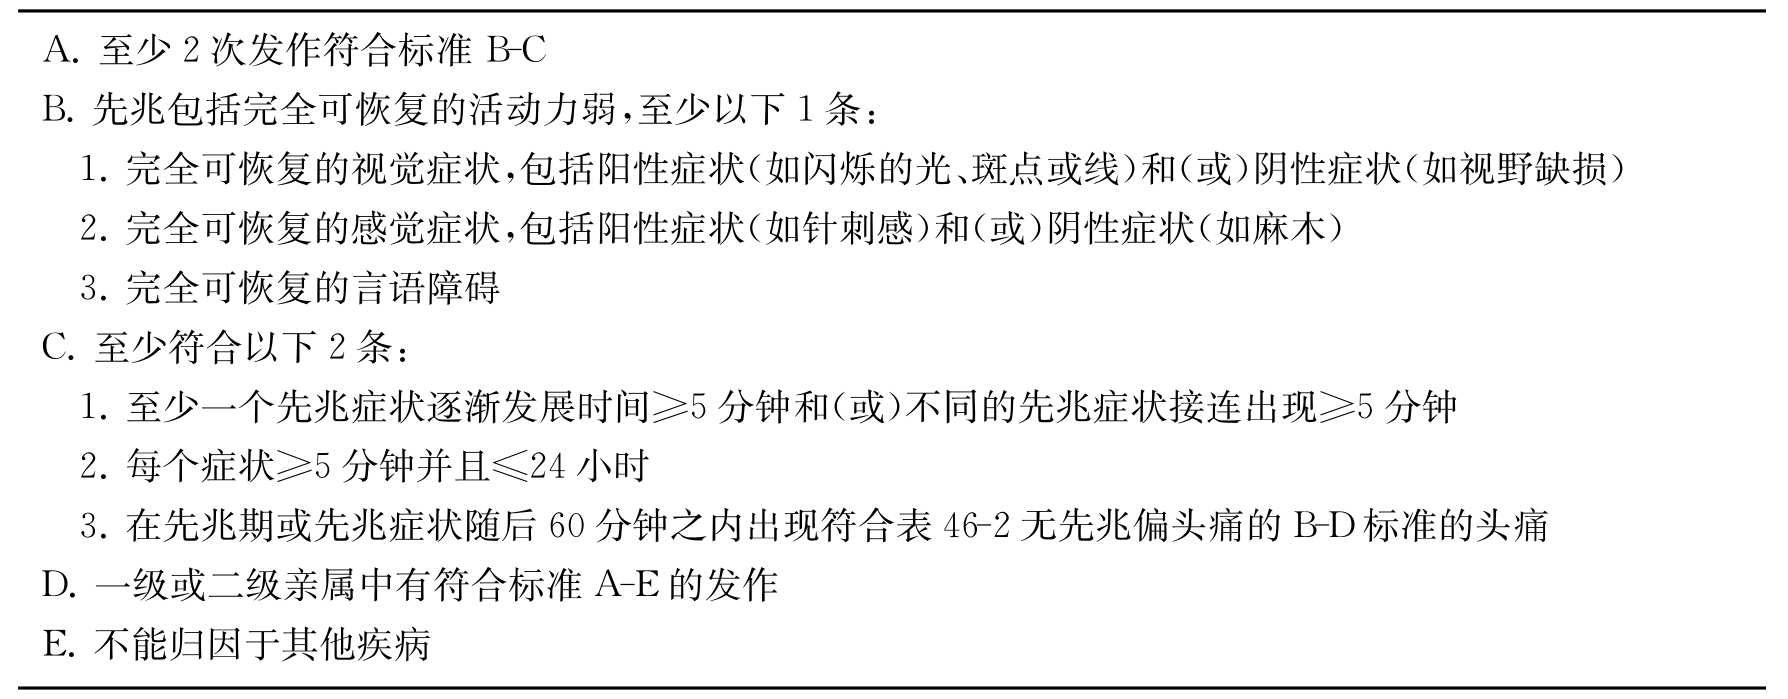
\includegraphics[width=5.94792in,height=2.32292in]{./images/Image00283.jpg}
\end{table}

\begin{table}[htbp]
\centering
\caption{散发性偏瘫性偏头痛的诊断标准}
\label{tab46-8}
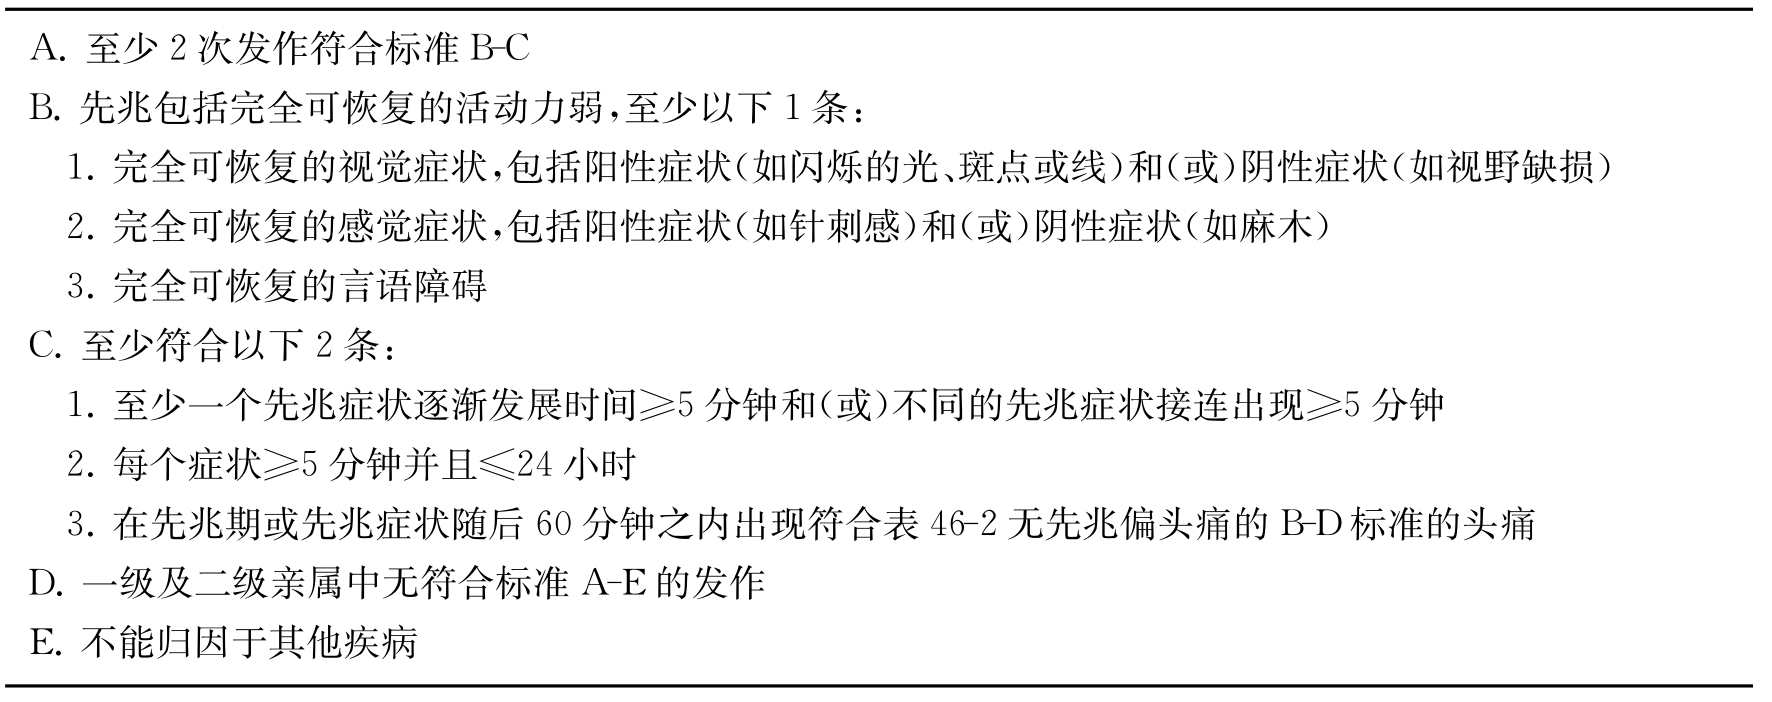
\includegraphics[width=5.89583in,height=2.33333in]{./images/Image00284.jpg}
\end{table}

\begin{table}[htbp]
\centering
\caption{基底型偏头痛的诊断标准}
\label{tab46-9}
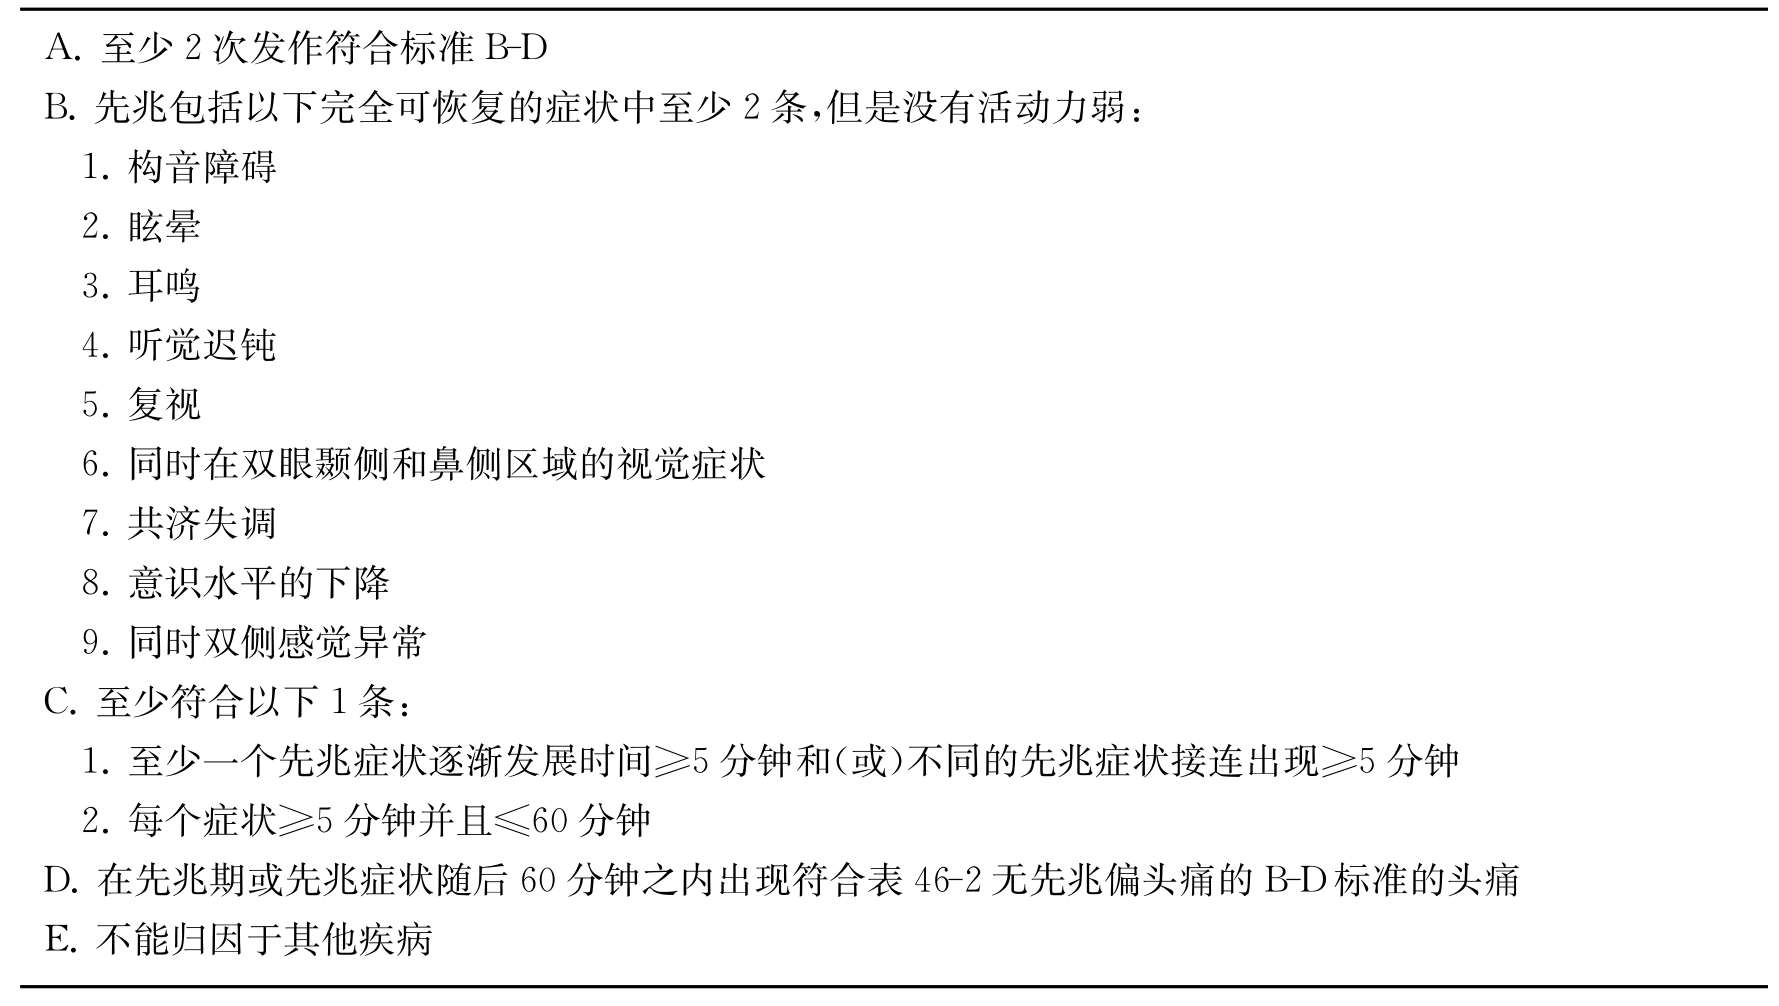
\includegraphics[width=5.91667in,height=3.34375in]{./images/Image00285.jpg}
\end{table}

\subsubsection{(三)常为偏头痛前驱的儿童周期性综合征}

常为偏头痛前驱的儿童周期性综合征包括下列3种类型:

\paragraph{1.周期性呕吐(cyclical vomiting)}

是儿童期一种阵发性自限性疾病,临床特征与偏头痛头痛的伴随症状类似。诊断标准是:①至少有5次发作符合标准②和③;②阵发性发作的严重恶心及呕吐,个别患儿常有其固定模式的发作,持续1小时至5天;③发作期间1小时内呕吐至少4次,且至少持续1小时;④两次发作间期症状完全缓解;⑤不能归因于其他疾病。

\paragraph{2.腹型偏头痛(abdominal migraine)}

是一种原因不明、主要发生于儿童的复发性疾病。诊断标准是:①至少有5次发作符合标准②~④;②腹痛持续1~72小时(未经治疗或治疗失败);③腹痛具备下列所有特征:位于腹部中线、脐周或难以定位,钝痛或疼痛性质难以描述,中或重度;④腹痛期间至少有下列两项发生:食欲缺乏、恶心、呕吐、脸色苍白;⑤不能归因于其他疾病。此外,本型发作有时伴随血管运动症状(面部潮红),大部分患儿日后会发生偏头痛。

\paragraph{3.儿童期良性发作性眩晕(benign paroxysmal vertigo of childhood)}

特征是在健康儿童反复短暂性眩晕发作,发作常伴随眼震或呕吐,有些发作会有单侧搏动性头痛,眩晕可突然发生和迅速缓解。诊断标准是:①至少有5次发作符合标准②;②无先兆多次严重眩晕发作,数分钟到数小时后自行缓解;③发作间期神经系统检查和听力、前庭功能正常;④脑电图正常。

确立上述三种疾病的诊断需先排除胃肠道、肝胆以及肾脏等疾病,另外,这三种疾病的发作临床上极易误诊为腹型癫痫或间脑癫痫。

\subsubsection{(四)视网膜性偏头痛(retinal migraine)}

是反复发作的单眼视觉障碍,包括闪烁、暗点或失明,并伴随偏头痛。诊断标准是:①至少有2次发作符合标准②和③;②单眼完全可逆性阳性和(或)阴性视觉症状(如闪烁、暗点或失明),在发作期间检查到或在适当指示下由患者描绘发作时的单眼视野缺陷来确定;③具有符合表\ref{tab46-2}无先兆偏头痛的B-D标准的头痛,后者开始于视觉症状发生时或发作过后60分钟内产生;④发作间期眼科检查正常;⑤不能归因于其他疾病。诊断本型头痛应排除其他会引起暂时性单眼失明的原因(黑蒙症),例如视神经病变或颈动脉剥离。

\subsubsection{(五)前庭性偏头痛(vestibular migraine,VM)}

是逐渐被人们了解的疾病,患者表现为发作性眩晕或不稳感,而这些患者在发病时或发病前同时具有偏头痛史。

VM可出现自发性或位置性眩晕。有些患者先出现一段时间的自发性眩晕,随后转为位置性眩晕。通常表现为旋转性而不是前后摆动的感觉,有些患者可能仅有或同时伴随更多的症状(如头晕、眼花、浮沉感、晕动病样感、头部游泳样或摇摆样感觉)。视觉性眩晕是VM的另一主要特征,是身处移动变换的场景(商业区、电影院)中诱发产生的眩晕。同时伴发恶心和平衡失调,但并非VM发作的特异性症状。

头痛的部位和严重程度变换多样。眩晕发生往往在偏头痛发作期,但也可发生在偏头痛间期或前期。约半数患者从未在眩晕发作期出现过头痛症状。一些患者(48\%)VM发作期仅表现为偏头痛症状。畏光、畏声、恐嗅和视觉或其他先兆,是VM最常见的伴随症状,这些对于诊断极为重要,眩晕的患者出现偏头痛先兆更加证实诊断的确切性。无先兆的偏头痛患者较有先兆者,更容易发生VM。一般患有VM的围绝经期女性仅表现为眩晕,而无偏头痛症状。

偏头痛通常与其他原因导致的发作性眩晕症状相混淆,如梅尼埃病和良性发作性位置性眩晕(BPPV)。VM的眩晕症状在头部保持一定位置时持续存在,而BPPV仅存在数秒钟。后循环缺血与VM的重要鉴别点为发作时畏光或畏声等偏头痛先兆症状,而其主要临床特点包括血压、血脂和(或)血糖异常、血管超声有动脉粥样硬化以及突然起身眼前发黑或头晕等。

\subsubsection{(六)月经性偏头痛}

月经性偏头痛是一种与卵巢周期变化有关的特殊类型偏头痛,多为无先兆偏头痛,发作通常持续时间较长,可达4~5天,与月经持续时间相当。可分为单纯性月经性无先兆偏头痛(pure
menstrual migraine,PMM)和月经相关性无先兆偏头痛(menstrually related
migraine,MRM)。PMM指无先兆的偏头痛只发生在围经期的5天里,即月经前2天至月经发生后3天,且至少在3个月经周期中有2个周期发生。MRM指无先兆的偏头痛不仅发生在围经期的5天里也发生在该月经周期的其他时间里。约46\%的女性偏头痛是MRM,14\%的女性偏头痛是PMM。

\subsubsection{(七)儿童偏头痛}

偏头痛是儿科头痛中常见病因之一,6~12岁儿童偏头痛发病率大约为2\%~5\%,青春期后渐增多,14岁左右发病率达10\%。

儿童偏头痛与成人相比有其特征性:①多为无先兆偏头痛发作类型;②头痛发作持续时间相对较短,而发作相对较频繁,患儿中有不少发作时间在1小时以内,甚至半小时左右;③头痛搏动性特点不突出;④头痛位于双侧较单侧常见;⑤畏光或畏声情况常见,胃肠道症状突出,伴有恶心、呕吐、腹痛者远较成人多;⑥约20\%的患儿在头痛之前或头痛时,逐渐出现视觉先兆,表现为双眼经常可见到光点、色彩、亮点或光线,偶尔也可发生在单眼,持续时间通常不超过30分钟。

儿童偏头痛需注意与头痛性癫痫相鉴别。小儿偏头痛脑电图(EEG)可以异常,因此对EEG异常的头痛患儿,应随访排除头痛性癫痫。其主要鉴别点为头痛性癫痫发作时可有意识改变或伴有其他类型癫痫表现,EEG有“痫样放电”。

\subsubsection{(八)偏头痛并发症(complication of migraine)}

包括下列几种情况:

\paragraph{1.慢性偏头痛(chronic migraine)}

由于慢性偏头痛病例大部分是由无先兆偏头痛开始,因此可将慢性偏头痛视为发作性偏头痛的并发症。其定义是指在没有药物过度使用的情况下,至少3个月偏头痛发作每月达到或超过15天;头痛的特点符合无先兆偏头痛的特点(表\ref{tab46-10})。

\begin{table}[htbp]
\centering
\caption{慢性偏头痛的诊断标准}
\label{tab46-10}
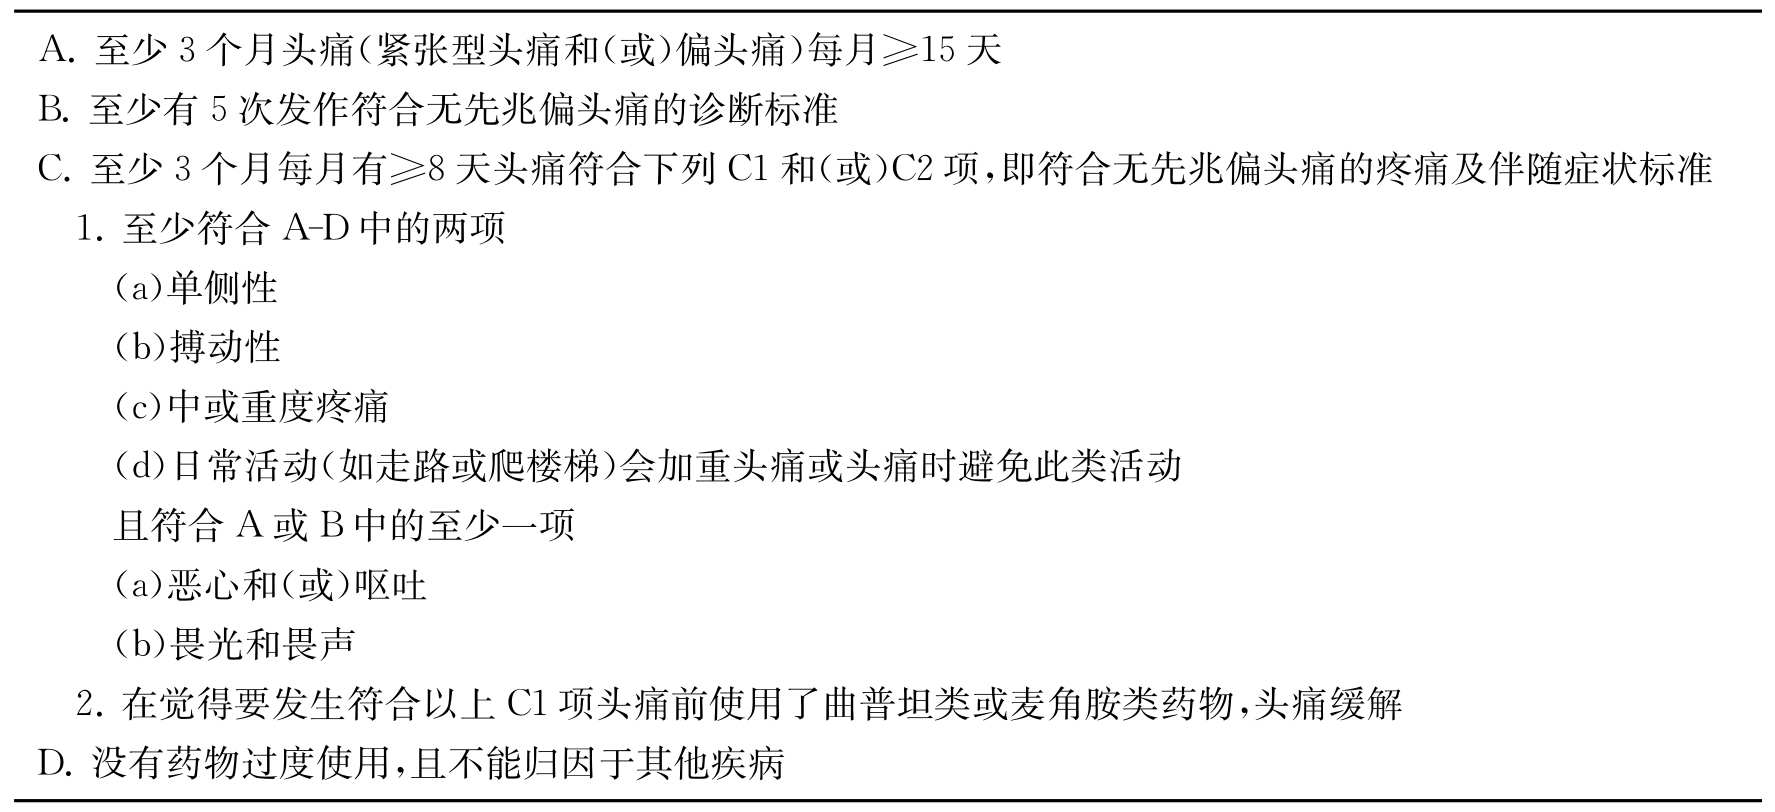
\includegraphics[width=5.90625in,height=2.69792in]{./images/Image00286.jpg}
\end{table}

\paragraph{2.偏头痛持续状态(status migrainosus)}

是一种使人极度失能的偏头痛发作,程度重,持续超过72小时(表\ref{tab46-11})。

\begin{table}[htbp]
\centering
\caption{偏头痛持续状态的诊断标准}
\label{tab46-11}
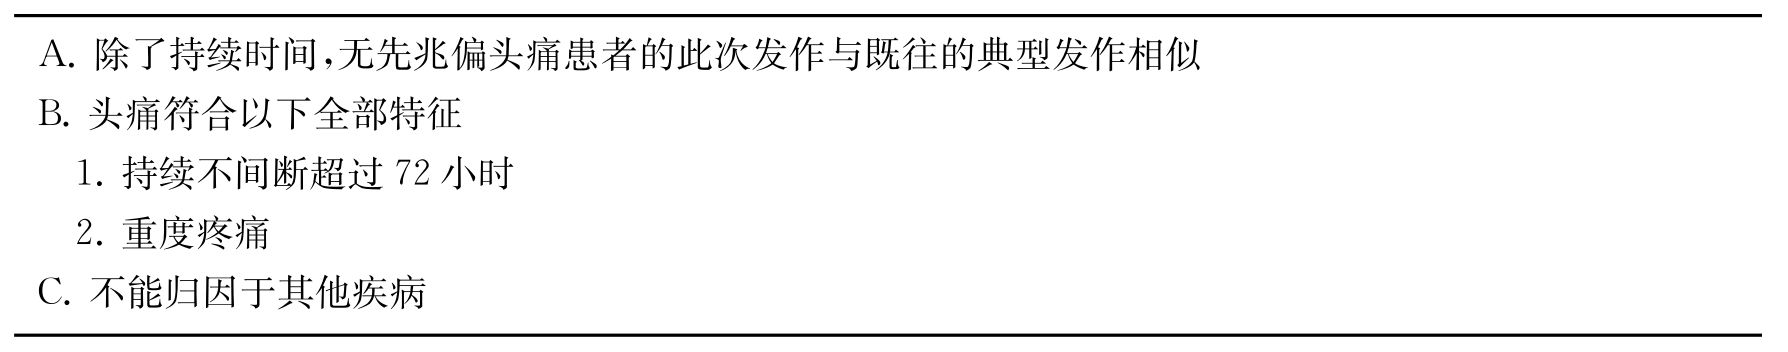
\includegraphics[width=5.94792in,height=1.16667in]{./images/Image00287.jpg}
\end{table}

\paragraph{3.不伴脑梗死的持续性先兆(persistent aura without infarction)}

本病罕见,是指有先兆偏头痛患者在本次发作中除一种或更多先兆症状持续超过1周外,其他情况和以前典型发作相同。发作通常为双侧,而且可能持续数月或数年之久。尽管乙酰唑胺(acetazolamide)和丙戊酸对少数患者有帮助,但本病有效治疗方法仍未知。

\paragraph{4.偏头痛性脑梗死(migrainous infarction)}

是指有先兆偏头痛患者在本次发作中除一种或更多先兆症状持续超过60分钟外,其他皆符合以前的典型发作,不同的是本次发作还出现与先兆症状一致的大脑区域缺血病变,且经由神经影像学证实为缺血性脑梗死。偏头痛患者发生缺血性脑卒中的可能情况有:偏头痛合并其他原因引发的脑梗死、其他原因的脑梗死而症状类似有先兆偏头痛、在典型有先兆偏头痛发作当中发生了脑梗死,只有最后一种才符合偏头痛性脑梗死的诊断。目前大量研究证实,偏头痛是缺血性卒中的危险因素。偏头痛,尤其是有先兆偏头痛和年龄<45岁的女性偏头痛会增加脑卒中的风险,但在男性及老年女性结论尚不一致。

\paragraph{5.偏头痛诱发型癫痫(migraine triggered seizure)}

系由偏头痛先兆触发的癫痫发作。偏头痛和癫痫是脑部发作性疾病的典型例子,类似偏头痛的头痛常在癫痫发作后产生,有时则是偏头痛发作中或发作后发生癫痫发作,这种现象有时称为偏癫痫(migralepsy)。在此亚型中,偏头痛发作符合有先兆偏头痛的诊断标准,癫痫发作则符合癫痫发作诊断标准中的某一类型,并在先兆偏头痛发作期间或发作后1小时以内发生。

偏头痛的鉴别诊断:偏头痛首要与颅内动脉瘤、动静脉畸形(arteriovenous
malformation,AVM)鉴别,后两者的头痛性质类似偏头痛但有时并非搏动性,而是胀痛、牵拉痛或其他;不一定伴有恶心、呕吐;动脉瘤的疼痛偶尔伴该侧动眼神经麻痹而出现复视,应注意与基底型偏头痛区别;偶尔先兆延长的发作可见于脑膜血管瘤。动静脉畸形在频发头痛前常有癫痫发作。偏头痛因其单侧性易误诊为三叉神经痛,但两者的疼痛性质迥异,前者为搏动性痛而后者为尖锐、电击样痛;发作时前者往往伴有恶心、呕吐、畏光或畏声,后者则多伴有流泪、面肌抽搐。

\protect\hypertarget{text00348.html}{}{}

\subsection{二、紧张型头痛}

紧张型头痛(tension-type
headache,TTH)旧称紧张性头痛、肌收缩性头痛、心因性头痛、神经性头痛、精神性头痛、压力性头痛等。它是指双侧颈枕部或全头部紧缩性或压迫性头痛,常与情绪障碍或心理因素有关,不伴恶心、呕吐等症状,可伴颈项部僵硬感,头痛呈持续性、波动性或阵发性。紧张型头痛是慢性头痛中最常见的一种,占慢性头痛的40\%,不同研究显示一般人口的终身患病率为30\%~78\%。诱因包括口及腭部的功能异常、心理或社会应激、惊恐、抑郁、妄想、肌肉紧张、紧张型头痛治疗药物的过量使用以及其他器质性病变影响等。

一向认为本型头痛主要是心因性所致,但近年不少研究提示本型头痛有其神经生物学基础,其发病有周围性以及中枢性机制的参与。本型头痛患者颅周肌筋膜组织压痛程度及肌筋膜触发点数目均明显增加,进而肌筋膜疼痛感受器敏化或周围激活促使疼痛敏感性增加。周围性机制对于发作性紧张型头痛具有极大重要性。敏感颅周肌筋膜组织接收到延长的疼痛信息,致使节段性中枢敏化,包括高颈段脊髓后角/三叉神经核水平,然后继发上位脊髓神经元的敏化,促使发作性紧张型头痛慢性转化。其他的因素如焦虑、抑郁可进一步加重中枢敏化。

紧张型头痛多在20岁左右起病,随年龄增长发病率增加,两性均可患病,女性多见。典型的紧张型头痛位于双侧头部,呈压迫感、紧缩感,每次头痛发作持续数十分钟至数日,程度轻至中度,不随日常活动加重,因此不至于导致日常生活障碍,这是和偏头痛在鉴别上的重要区别。除了慢性紧张型头痛可以伴有轻度恶心之外,一般无恶心、呕吐,但可有食欲缺乏。光或声音刺激有时是加重因素。

触诊检查颅周压痛增强:触痛肌肉部位的肌肉敏感性和硬度源于局部挛缩,需触诊检查颅周肌筋膜压痛程度和扳机点位置来发现痛源,在额肌、颞肌、咬肌、翼内外肌、胸锁乳突肌、夹肌、斜方肌上用力压迫,会加重头痛的强度和频率以及头痛的高峰。

依其发作频度以及是否伴有颅周压痛分为以下几型:

\subsubsection{(一)偶发性发作性紧张型头痛(infrequent episodic tension-type}
headache)

是指头痛平均每月发作少于1日(每年少于12日),至少有10次以上发作。根据压痛实验是否阳性,可以细分为“偶发性发作性紧张型头痛伴颅周压痛”和“偶发性发作性紧张型头痛不伴颅周压痛”(表\ref{tab46-12})。

\subsubsection{(二)频发性发作性紧张型头痛(frequent episodic tension-type headache)}

是指头痛经常发作,平均每月≥1日但<15日,已至少3个月(每年≥12日且<180日),至少有10次以上发作。根据压痛实验是否阳性,可以细分为“频发性发作性紧张型头痛伴颅周压痛”和“频发性发作性紧张型头痛不伴颅周压痛”(表\ref{tab46-12})。此型头痛多伴无先兆偏头痛。

\subsubsection{(三)慢性紧张型头痛(chronic tension-type headache)}

是由发作性紧张型头痛演变而来,每日或非常频繁地发作,平均每月>15日(每年>180日),已至少3个月。根据压痛实验是否阳性,可以细分为“慢性紧张型头痛伴颅周压痛”和“慢性紧张型头痛不伴颅周压痛”(表\ref{tab46-12})。此型头痛就医比例较高,有药物依赖倾向。

若头痛符合慢性紧张型头痛诊断标准,且明确地于第一次发生后3天内,头痛即每日发作且无缓解,则诊断为新发每日持续性头痛(new
daily-persistent
headache,NDPH),但如开始发作的情形不记得或不确定时,则诊断为慢性紧张型头痛。

\begin{longtable}{c}
 \caption{紧张型头痛的诊断标准}
 \label{tab46-12}
 \endfirsthead
 \caption[]{紧张型头痛的诊断标准}
 \endhead
 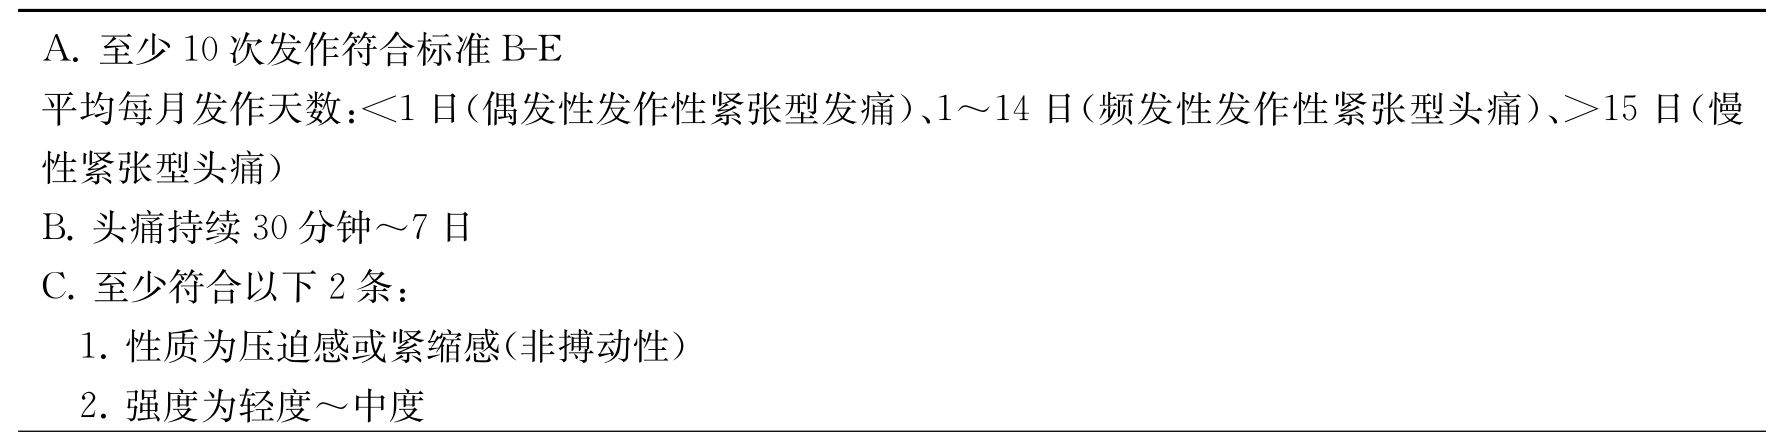
\includegraphics[width=\textwidth,height=\textheight,keepaspectratio]{./images/Image00288.jpg}\\
 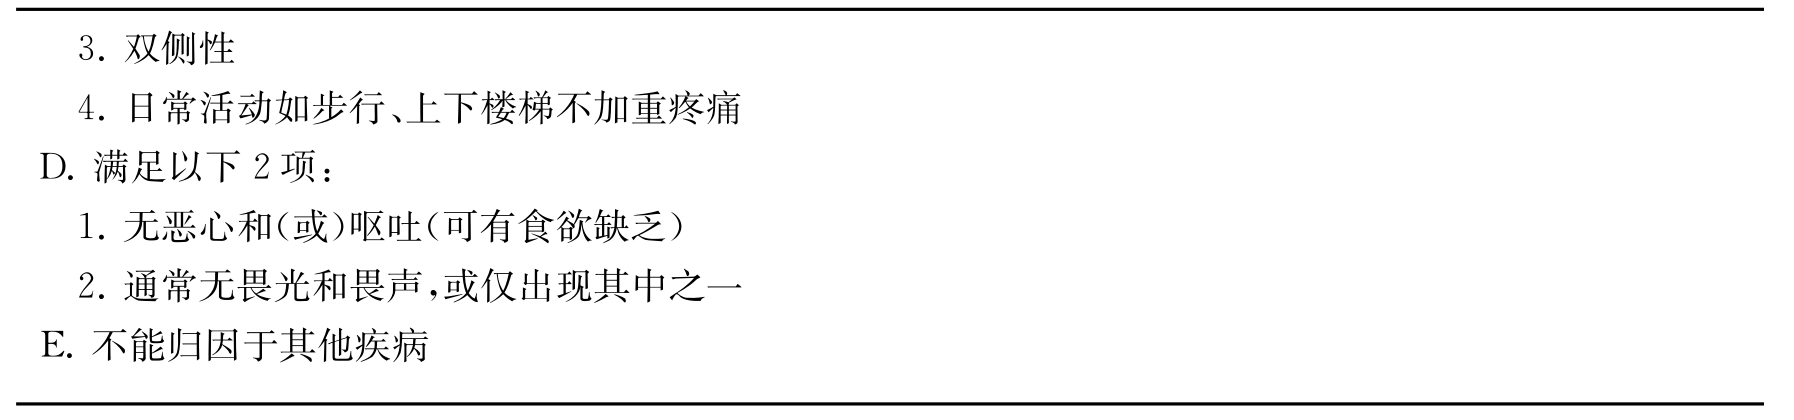
\includegraphics[width=\textwidth,height=\textheight,keepaspectratio]{./images/Image00289.jpg}
 \end{longtable}

\protect\hypertarget{text00349.html}{}{}

\subsection{三、丛集性头痛}

丛集性头痛(cluster
headache)是一种局限于单侧的以眶、颞、额等区为主的严重发作性疼痛并伴有同侧的自主神经症状的原发性头痛,具有典型的周期性,在丛集期内头痛密集发作,因而得名。包括两种类型,即发作性丛集性头痛(episodic
cluster headache,ECH)和慢性丛集性头痛(chronic cluster
headache,CCH)。ECH有自限性发作周期,所谓丛集期一般持续7天~1年,间歇期不少于1个月,通常为数月至数年。CCH特点为1年内无间歇期或间歇期少于1个月,发作频率增加或对药物治疗不敏感。CCH可由初次发作就持续无缓解,称为原发性慢性丛集性头痛,也可由ECH发展而来,称为继发性慢性丛集性头痛。最少见的是继发性发作性丛集性头痛,即由慢性发展为发作性。ECH和CCH都会持续数年,两者可互相转化。ECH的间歇期可能持续很多年,但患者直到老年才会停止复发。

至今仍缺乏对丛集性头痛发病机制统一的解释。任何假设都必须解释该疾患的3个基本特征:周期节律性、疼痛以及自主神经表现。有模型对丛集性头痛的发病机制进行总结,即在一易感时间,即“丛集期”内,丛集性头痛的发作由一个功能异常的下丘脑节拍器起步,来自中枢或周围的触发因素激活硬脑膜的三叉神经血管和头颅副交感神经系统,在脑干和脊髓中下丘脑与泌涎核和副交感神经核、节前交感神经元有明确的功能联系,这些通路的激活导致海绵窦痛性血管的改变,继而颈动脉海绵窦段的交感神经丛参与进来,刺激泪腺和其他黏膜腺体的分泌功能。

丛集性头痛主要为男性多发,有报道男女比例约为9∶1,人群中患病率约为0.1\%~0.4\%。发病年龄多为20~40岁,儿童及70岁以上老年人很少见。郭述苏等于1986年对我国26个省、自治区进行丛集性头痛流行病学调查,显示患病率6.8/10
0000,男女比例为6.2∶1,总体认为,中国丛集性头痛患病率较低,CCH患病率低于ECH。

丛集性头痛发作的典型特征是突然发作而无任何先兆。10~15分钟达高峰,一般持续30~45分钟,按国际头痛协会(IHS)诊断标准,可持续15~180分钟,发作频率不等,从2天发作1次至1天发作8次或更多。头痛通常局限在单侧,最常见的部位按发作频率高低依次为眼眶、眶后、颞部、眶上和眶下。对于大多数患者而言,疼痛先起自眶窝和附近区域,或起自三叉神经第一支分布区,随后扩展至同侧额部、颞部、耳周和鼻区,还可扩展至同侧肩部和颈部区域。丛集性头痛是最严重的头痛,患者常描述钻痛或撕裂样疼痛、非搏动性烧灼样疼痛。在任何丛集期,头痛始终发生在同一侧,甚至每年都在同侧,偶尔头痛位于对侧,左右两侧交替出现极少见。

发作的周期如同钟表一样规律,头痛可在每年同一季节发作。头痛常在每天的同一时间发作,有些患者头痛发作时间出奇的准确。头痛大部分发生在休息时,如在工作一天后回家的路上,许多患者在入睡大约2小时后的快速眼动(REM)睡眠期会痛醒,头痛也可发生在非快速眼动(NREM)期。睡眠呼吸暂停和氧饱和度下降可能诱发发作。有时每晚头痛发作3~4次使患者无法睡眠,导致白天打盹,出现更严重的头痛发作。

头痛发作时可伴有一个或多个以下的伴随症状:结膜充血、流泪、鼻塞、流涕、前额和面部出汗、瞳孔缩小、眼睑下垂和眼睑水肿,还经常伴有面部发红或苍白、头皮和面部触痛、颈动脉压痛等症状,并且均为同侧发作。多数认为不会出现恶心、呕吐,但一个针对中国人丛集性头痛的调查发现60\%患者有恶心,41.7\%的患者畏光,40.8\%的患者畏声。与有自主神经症状的患者相比,无自主神经症状的患者剧烈发作的次数少。在无自主神经症状的患者中,女性患者和慢性患者有更高的发作频率。

在丛集性头痛发作期,患者有烦躁感或易怒、行为怪异、咆哮、哭叫,甚至会自杀。多数患者会不停来回走动以缓解头痛,少数与偏头痛患者一样,喜欢在黑暗安静的环境中独处。许多患者会用手、冰袋或热毛巾压住眼睛或颞部。头痛发作后,患者常筋疲力尽。有的患者害怕入睡后再次头痛发作,宁愿彻夜不眠,当睡意最终无法克服时,会导致患者迅速进入REM期睡眠,入睡后数分钟头痛再次发作。

在丛集期患者对某些物质特别敏感,如酒精和血管扩张剂(硝酸甘油、组胺),而在间歇期这些物质很少诱发头痛。与偏头痛不同,任何形式的酒精(包括啤酒、烈酒、葡萄酒等)都可诱发丛集性头痛。酒精也许仅作为血管扩张剂发挥其作用,但目前尚不明确。与偏头痛不同,食物类型及对某种食物嗜好不会诱发丛集性头痛发作。丛集性头痛患者中吸烟的比例较高,一些患者戒烟后头痛得到缓解,但吸烟不像酒精那么敏感。近来又发现一种新的诱发因素-体温升高。由于环境、热水浴、中枢性发热、劳作、性交等,可在约1小时内诱发,有患者在夏季度假时出现了新的丛集期。一般建议患者保持室内温度凉爽,并尽量避免其他可能增加体温的因素,这样可明显降低从集期的发作频率和严重程度。

丛集性头痛的诊断主要是临床诊断,其中头痛迅速加剧、夜间发作明显、每次头痛持续时间短等病史是诊断的重要依据,必要的神经影像学检查有助于排除颅内器质性病变。

\subsubsection{(一)丛集性头痛的诊断标准(表\ref{tab46-13})}

\begin{table}[htbp]
\begin{centering}
\caption{丛集性头痛的诊断标准}
\label{tab46-13}
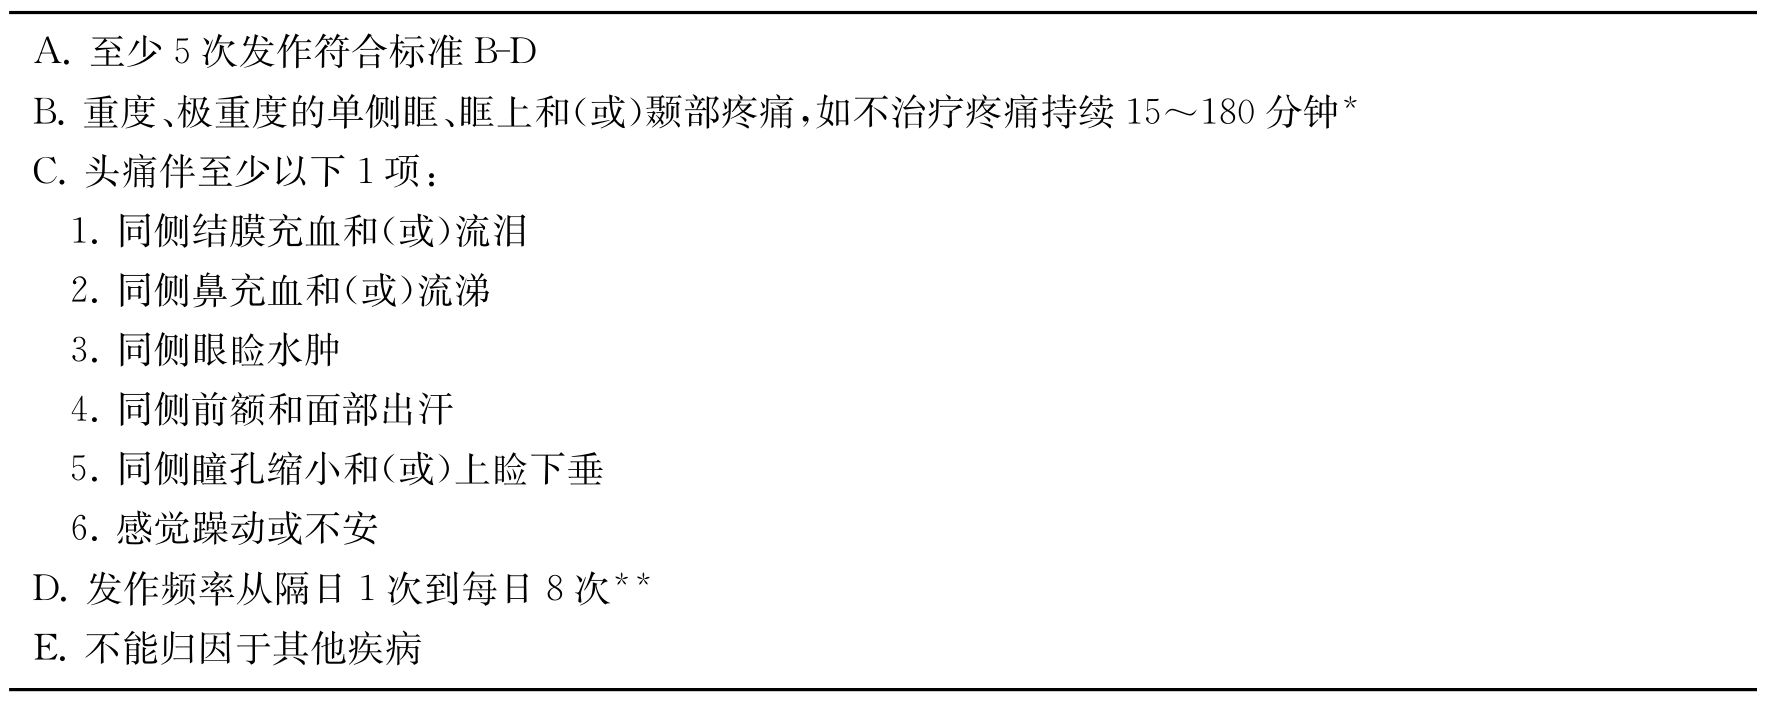
\includegraphics[width=5.9375in,height=2.33333in]{./images/Image00290.jpg}
\end{centering}

{\small 注:

*:丛集性头痛的发作间期(但不超过发作期的1/2),可能会有头痛程度减轻,和(或)持续时间的改变(缩短或延长);

**:丛集性头痛的发作间期(但不超过发作期的1/2),可能会有发作频率的下降。}
\end{table}



\subsubsection{(二)丛集性头痛的分类及诊断标准(表\ref{tab46-14})}

\begin{table}[htbp]
\centering
\caption{丛集性头痛的分类及诊断标准}
\label{tab46-14}
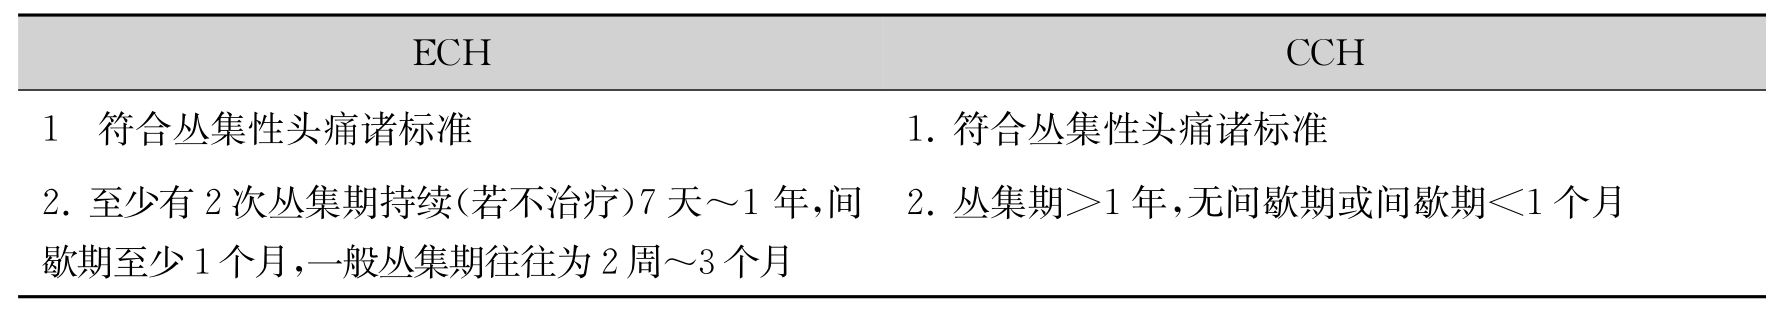
\includegraphics[width=5.9375in,height=1.04167in]{./images/Image00291.jpg}
\end{table}

按诊断标准ECH与CCH发作时临床表现相似,仅有缓解期起始与持续时间不同。但最近发现两者有一定临床差异:①与ECH相比,CCH在两次发作间更多出现轻度持续性头痛;②ECH疼痛部位主要为眶后及颞部,且头痛始终发生在同一侧,但CCH也可有上齿、颚部、面颊、耳、肩部疼痛及疼痛部位的左右换位;③ECH、CCH最常见的自主神经症状均为流泪,但CCH鼻溢症状较少,而恐嗅症出现较多;④CCH发作持续时间较ECH短。

\subsubsection{(三)鉴别诊断}

\paragraph{1.常见原发性头痛的鉴别(表\ref{tab46-15})}

\begin{table}[htbp]
\centering
\caption{常见原发性头痛的鉴别}
\label{tab46-15}
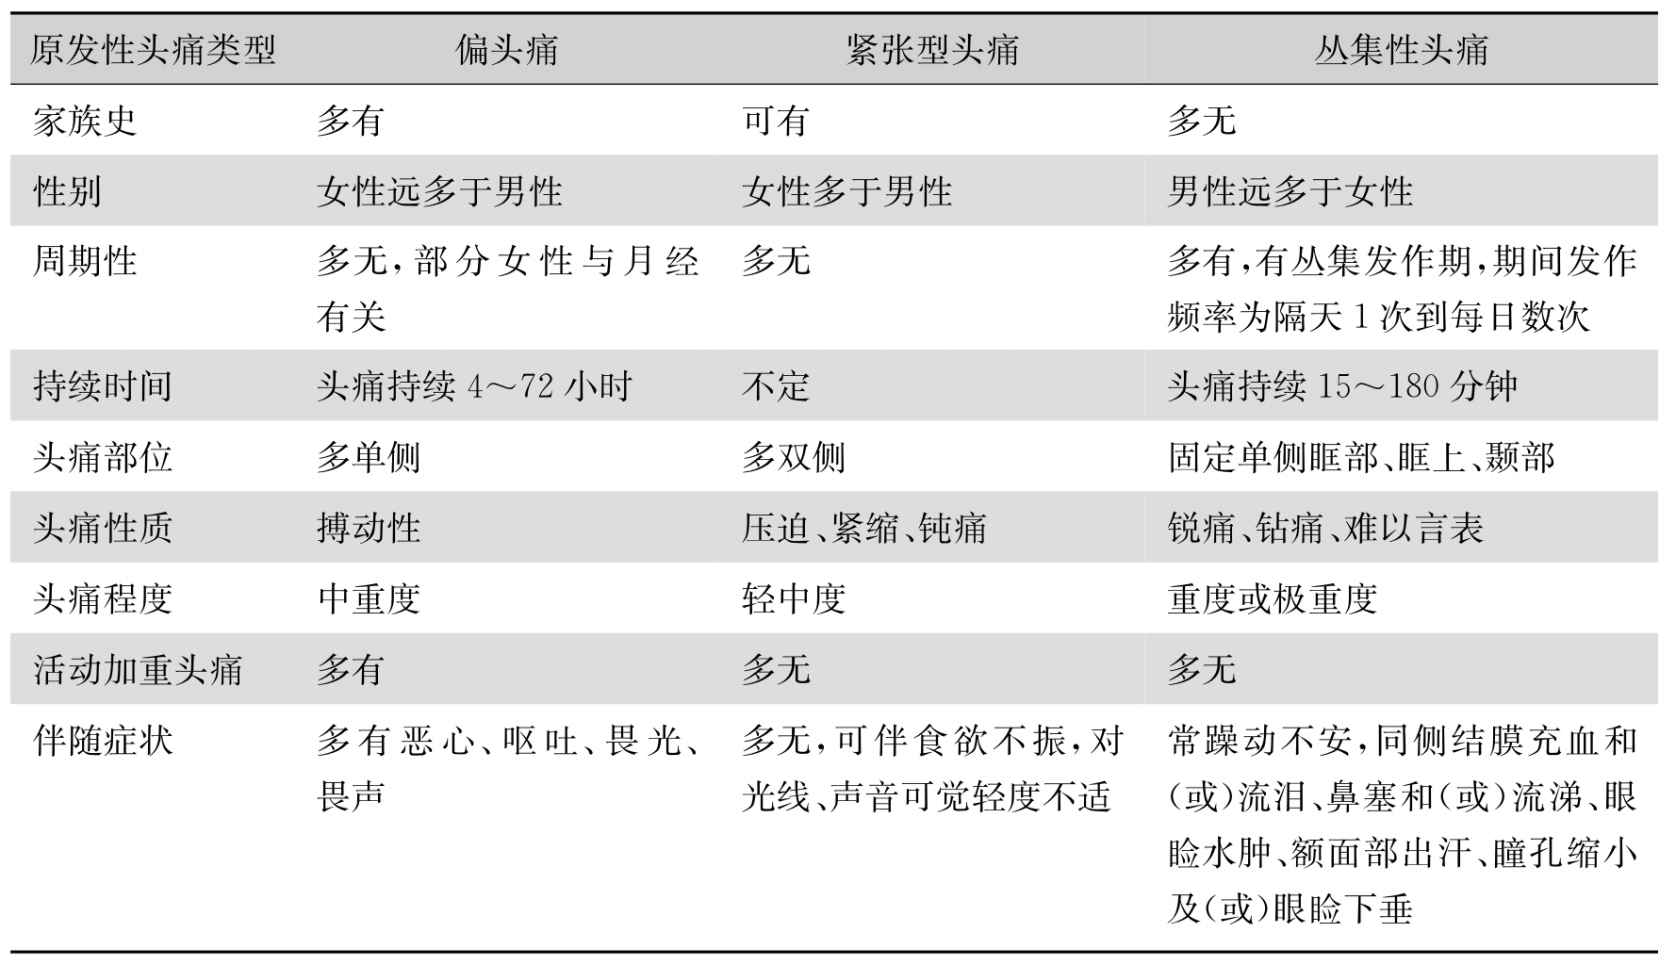
\includegraphics[width=5.91667in,height=3.40625in]{./images/Image00292.jpg}
\end{table}

\paragraph{2.持续时间短暂的头痛的鉴别(表\ref{tab46-16})}

\begin{longtable}{c}
 \caption{持续时间短暂的头痛的鉴别}
 \label{tab46-16}
 \endfirsthead
 \caption[]{持续时间短暂的头痛的鉴别}
 \endhead
 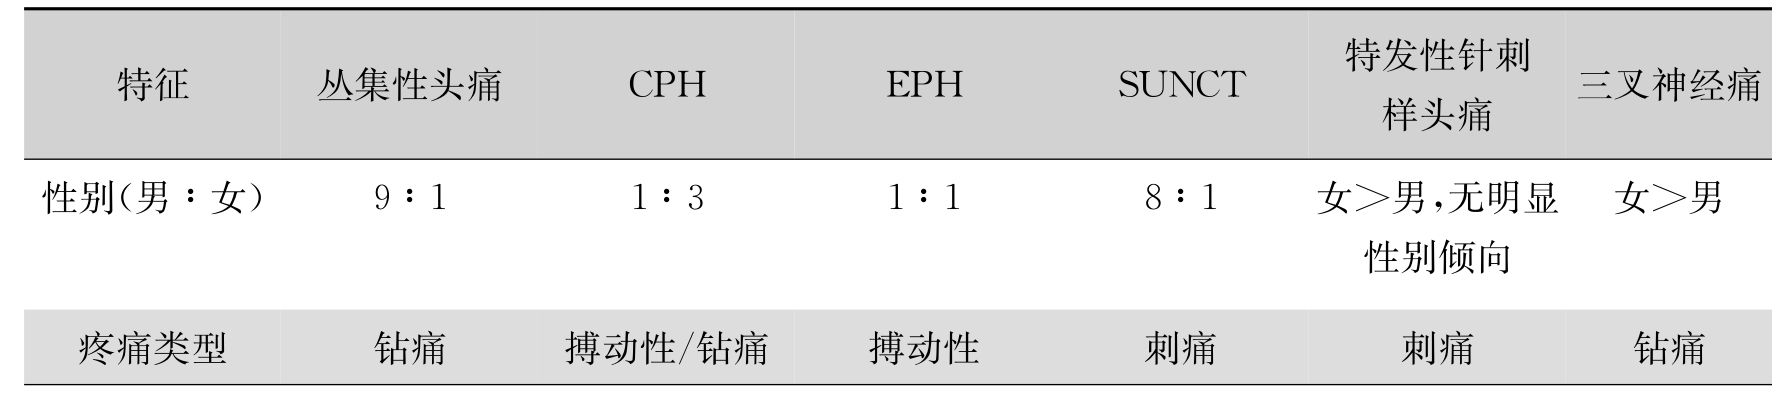
\includegraphics[width=\textwidth,height=\textheight,keepaspectratio]{./images/Image00293.jpg}\\
 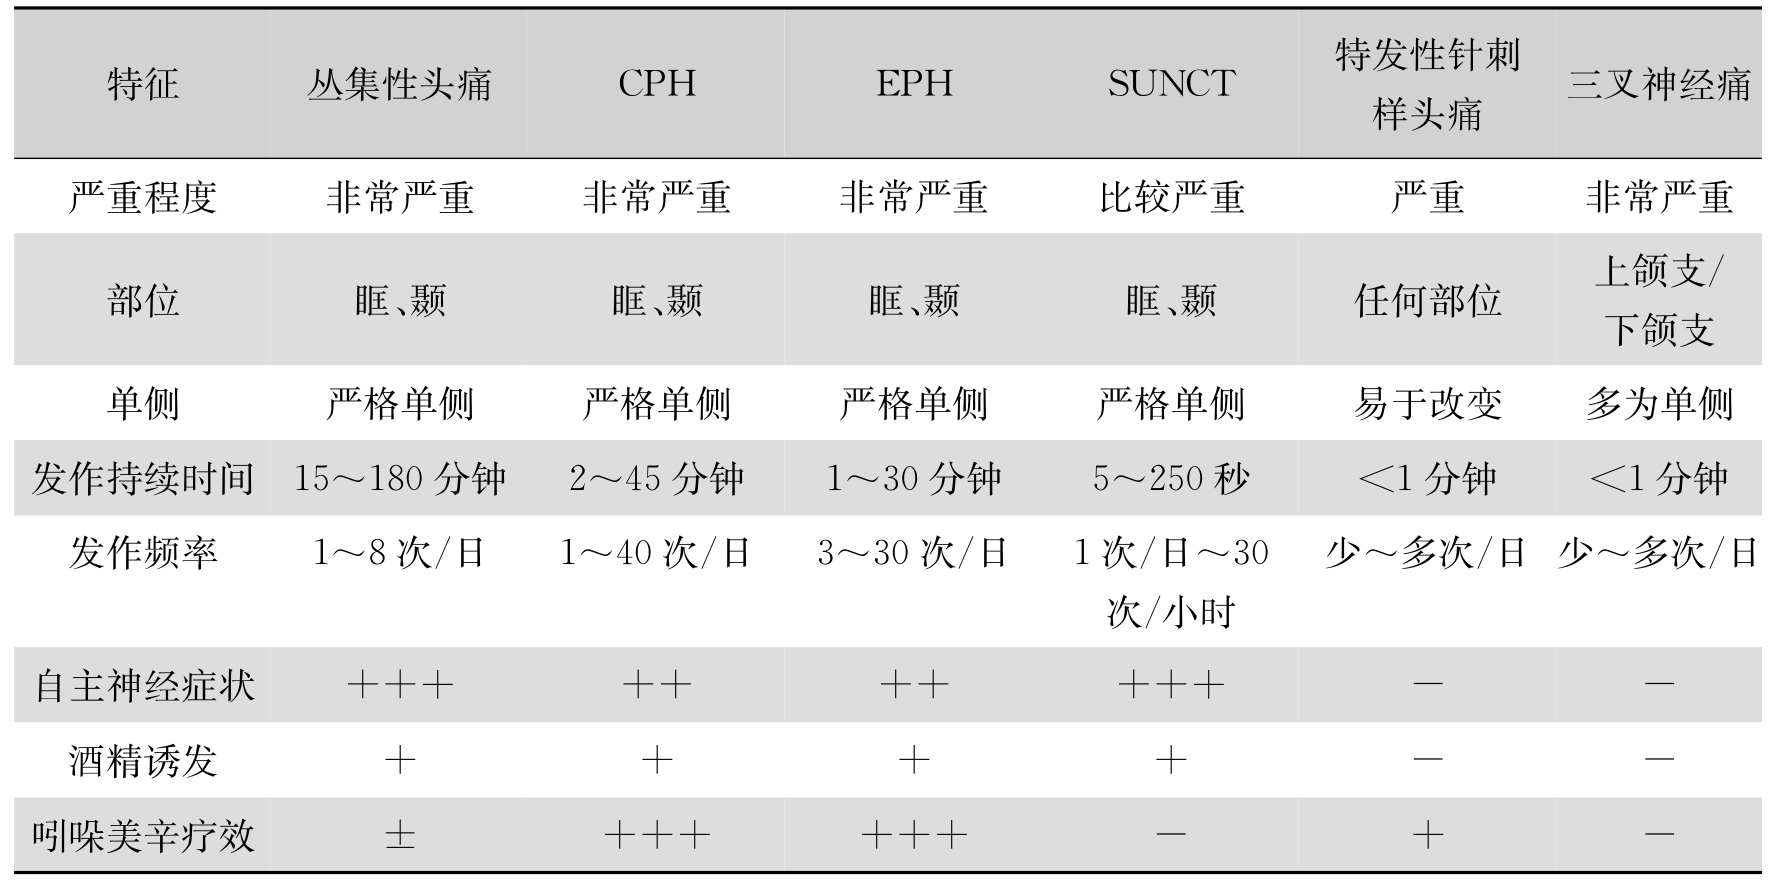
\includegraphics[width=\textwidth,height=\textheight,keepaspectratio]{./images/Image00294.jpg}
 \end{longtable}

注:CPH:慢性发作性半边头痛(chronic paroxysmal
hemicrania);EPH:阵发发作性半边头痛(episodic paroxysmal
hemicrania);SUNCT:短暂单侧神经痛性头痛发作并结膜充血及流泪(short-lasting
unilateral neuralgiform headache attack with conjunctival injection and
tearing);

特发性针刺样头痛:可与偏头痛、丛集性头痛、紧张型头痛及外伤后头痛伴发,也可以是一个独立的疾病;三叉神经痛:面部存在扳机点,刺激该处可引起剧烈疼痛。三叉神经痛患者不愿触摸面部,而丛集性头痛患者却宁愿按压面部以缓解疼痛

\protect\hypertarget{text00350.html}{}{}

\subsection{四、其他三叉自主神经头痛}

三叉自主神经头痛(trigeminal autonomic
cephalgia)是指同时有头痛的临床特征及明显的颅部副交感神经症状,不同于后述的三叉神经痛。实验及人体FMRI检查显示这些综合征会激活正常人体的三叉神经、副神经反射,伴随继发性颅部交感神经功能异常。三叉自主神经头痛除了丛集性头痛以外,还包括发作性半边头痛、短暂单侧神经痛性头痛发作并结膜充血及流泪等。

\subsubsection{(一)发作性半边头痛(paroxysmal hemicrania)}

其特征、伴随症状和体征均与丛集性头痛相似,但持续时间较短(2~30分钟),且较频繁(在全部发作中,发作频率为每日5次以上者占了一半以上),头痛时至少伴随下列1项症状并位于同侧:①结膜充血及(或)流泪;②鼻腔充血和(或)流涕;③眼睑水肿;④前额及脸部出汗;⑤瞳孔缩小及(或)眼睑下垂。本病的特征之一是治疗量的吲哚美辛可完全预防发作。发作性半边头痛可分为:①阵发发作性半边头痛:至少有两次的发作周期为7~365日,其中间隔至少1个月的无痛缓解期;②慢性发作性半边头痛:反复发作长于1年而无缓解期或缓解。

\subsubsection{(二)短暂单侧神经痛性头痛发作并结膜充血及流泪(short-lasting unilateral}
neural giform headache attack with conjunctival injection and
tearing,SUNCT)

本综合征在近年内已被确认,其特征是短暂的单侧头痛发作,位于眼眶、上眼眶或颞部刺痛或搏动性疼痛,持续5~240秒,伴随同侧结膜充血及流泪,发作频率为每日3~200次。有文献指出,症状最类似SUNCT的颅内结构性疾患是位于颅后窝或侵犯脑垂体的病变,需注意鉴别。

\protect\hypertarget{text00351.html}{}{}

\subsection{五、其他原发性头痛}

其他原发性头痛(other primary
headache)包括临床上几种异质性疾病,对其发病机制仍了解很少。

\subsubsection{(一)原发性刺戳性头痛(primary stabbing headache)}

旧称冰淇淋头痛、冰锥痛、刺戳痛等。头痛的发生如同单一或连续的刺戳,主要或完全集中在三叉神经第一支分布区(眼窝、颞部及顶部),持续最多数秒,一天内出现一至很多次不规则发作,无伴随症状。如连续发作一周以上且局限于同一部位时,应详细检查该处有否结构性病变。

\subsubsection{(二)原发性咳嗽性头痛(primary cough headache)}

旧称良性咳嗽头痛、Valsalva操作性头痛。原发性咳嗽性头痛为突然发作,持续1秒钟至30分钟,仅由咳嗽、用力和(或)Valsalva手法诱发和加重。原发性咳嗽性头痛一般是双侧受累,一部分患者在伴有咳嗽的呼吸道感染后发作。咳嗽性头痛也包括由喷嚏、举重物弯腰屈身、用力排便等诱发的头痛。举重物也可导致急性双侧性项枕部或项枕顶部头痛,头痛可持续数天至数周,可能是牵拉了颈部的肌腱和韧带所致。应排除其他继发性原因,如蛛网膜下腔出血。原发性咳嗽性头痛的发病与颅内压升高有关,疼痛的确切病因仍不清。诊断此类头痛需经神经影像学检查除外结构性损害后方可考虑。

\subsubsection{(三)原发性劳力性头痛(primary exertional headache)}

又称良性劳力性头痛。原发性劳力性头痛由运动引起,只发生于运动期间或之后,持续5分钟至48小时,典型地为双侧搏动性疼痛,不能归因于其他疾病。目前报道的原因包括跑步、划船、打网球、游泳等运动。一种特定的运动对于某些人可以诱发头痛,而对其他人可无反应。运动可为某些偏头痛患者发作典型偏头痛的诱发因素。吲哚美辛对大部分患者有效。

\subsubsection{(四)与性行为相关的原发性头痛(primary headache associated with sexual}
activity)

是在没有任何颅内疾病的情况下,因性行为引起的头痛,通常在性兴奋增加时开始出现头部两侧钝痛,并在高潮时突然变为剧烈,可持续1分钟至3小时。性高潮前头痛是一种头和颈部的钝痛,与颈部的肌肉收缩有关,发生于性活动过程中,随着性活动的进行而加重。性高潮头痛是一种突然的、严重的、爆炸性头痛,在性高潮时出现。在极少数情况下,性活动能造成脑脊液漏,导致低脑脊液压力型头痛。对于首次出现的性交性头痛,诊断时要谨慎。因为囊状动脉瘤破裂的诱因中12\%与性行为有关,动静脉畸形所致的蛛网膜下腔出血的诱因中4\%与性行为有关。

\subsubsection{(五)睡眠性头痛(hypnic headache)}

是一种只在睡眠中发生、并使患者痛醒的头痛,为钝痛性质,多数双侧,通常为轻至中度,约20\%的患者为重度,一般持续15~180分钟,至少具有下列两项特征:①每个月内发作>15次;②醒来后持续≥15分钟;③首次发作在50岁之后。无自主神经系统症状,且恶心、畏光、畏声这三项症状中最多不超过一项。诊断本型头痛时应排除颅内结构性疾病,并注意与三叉自主神经头痛(trigeminal
autonomic cephalalgia)相鉴别。

\subsubsection{(六)原发性霹雳性头痛(primary thunderclap headache)}

突发的头痛,不到1分钟便可达到最严重的程度,其剧烈犹如破裂的脑动脉瘤头痛,持续1小时至10天,开始发病的一周内可能复发,但接下来的几周或几个月则表现为无规律性复发。诊断本型头痛除了这些临床特点以外还必须:①脑脊液和神经影像学检查均正常;②必须排除下列疾病:蛛网膜下腔出血、脑出血、大脑静脉栓塞、破裂的血管畸形(多数为动脉瘤)、动脉剥离(颅内及颅外)、中枢神经系统血管炎、第三脑室囊肿、低脑脊液压、急性鼻窦炎(尤其是气压性创伤所致者)等。

\subsubsection{(七)持续性半边头痛(hemicrania continua)}

是一种持续性且严格固定的单侧头痛,每天持续,没有无痛期,部位固定一侧(不换边),疼痛程度为中度,但可加剧至重度,在加剧期间至少会有下列1项自主神经症候出现在疼痛同侧:①结膜充血及(或)流泪;②鼻腔充血及(或)流涕;③眼皮水肿及(或)瞳孔缩小。对治疗量的吲哚美辛有效。除这些标准外,头痛必须持续大于3个月方能诊断为本型头痛。

\subsubsection{(八)新发每日持续性头痛(new daily-persistent headache,NDPH)}

旧称新发慢性头痛(de novo chronic
headache)、急性发作的慢性头痛(chronic headache with acute
onset)。本型头痛的诊断标准是:①头痛持续大于3个月,且符合标准②~④;②从开始发生或发生后少于3日内,头痛即每日发作且无缓解;③至少有下列两项疼痛特征:双侧;压迫/紧缩性(非搏动性);程度轻或中度;不会因日常活动如走路或爬楼梯而加剧;④下列两项皆符合:最多只有畏光、畏声或轻度恶心3项中的1项;没有中度或重度恶心,也没有呕吐;⑤不能归因于其他疾病。此外,本型头痛可有两种亚型:一是自我缓解亚型,典型者数月内在无治疗下自行缓解;另一为顽固性亚型,对积极的治疗有抗拒性。

\protect\hypertarget{text00352.html}{}{}

\section{155 继发性头痛}

\subsection{一、头和(或)颈部外伤的头痛}

头、颈或脑部外伤后常发生头痛,往往伴有其他症状如头晕、注意力难集中、神经质、人格改变和失眠,此群症状称为外伤后综合征(posttraumatic
syndrome),头痛是其中最突出的症状,且头痛的类型有多种,还可能和原发性头痛尤其是紧张型头痛相似而导致诊断的混乱。

\subsubsection{(一)轻微头部外伤和脑震荡后综合征的头痛}

轻微闭合性脑损伤经典定义如下:意识丧失30分钟以下或仅有头晕而无意识丧失;初始Glasgow昏迷评分在13~15分之间,无继续恶化;未发现凹陷性颅骨骨折及局灶神经体征;无颅内血肿或其他神经外科病变。脑震荡后综合征通常继发于轻微脑损伤,由一个或多个症状和体征组成,常表现为头痛、脑神经症状和体征、心理及躯体不适、认知受损以及少见的后遗症。最常见的主诉是头痛、头晕、疲劳、易怒、焦虑、失眠、注意力和记忆力丧失以及噪声过敏。意识丧失在脑震荡后综合征的发生中不是必须的。

根据国际头痛协会第二版分类标准,外伤后7天以内发生的头痛才是外伤后头痛。可出现多种类型的头痛:

\paragraph{1.紧张型头痛}

紧张型头痛约占外伤后头痛的85\%。头痛的分布范围多种多样,持续时间不同。通常描述为头部压痛、紧缩或钝痛。

\paragraph{2.枕神经痛}

疼痛的性质可为钝痛、紧缩感、刺痛或跳痛,疼痛的范围为颈枕部或顶、颞、额或眶周或眶后。头痛持续时间从数分钟、数小时至数天不等,单侧或双侧同时出现。

\paragraph{3.偏头痛}

反复发作的伴有或不伴有先兆的偏头痛亦可由轻微头部外伤引起。

\paragraph{4.丛集性头痛}

丛集性头痛也可由轻微头部外伤引起,但很少见。

\paragraph{5.眶上和眶下神经痛}

在闪电痛、麻刺感、刺痛或烧灼痛的同时,常伴有受损神经分布范围的感觉减退或改变,以及出汗减少。疼痛可为发作性或持续性,钝痛或跳痛也可发生在损伤的周围。

\subsubsection{(二)鞭击伤后头痛}

鞭击伤(whiplash)多见于交通事故,外力自背后或一侧经加速/减速机制,使能量转移至颈部而引起的损伤。临床表现主要是与颈部有关的症状和体征,还有颈部以外的症状,诸如躯体障碍、神经感觉障碍、行为和认知障碍、情感性疾病等。头痛在鞭击伤后综合征中很常见。鞭击伤后,约80\%的患者主诉头痛,头痛常为紧张型头痛,并常与枕大神经痛相伴随。半头棘肌、头上斜肌、头夹肌、头直肌、颈夹肌、上斜肌、胸锁乳突肌、咬肌、颜肌及枕额肌等肌肉上的触发点受到刺激时,常产生头部疼痛。

\paragraph{1.鞭击伤后急性头痛(acute headache attributed to whiplash injury)}

其诊断标准为:①头痛,无典型特征,符合标准③及④;②有鞭击伤病史(突然并显著的颈部加速/减速动作),当时伴随颈部疼痛;③头痛在鞭击伤后7日内发生;④有下列任何一项:头痛在鞭击伤后3个月缓解;头痛持续,但自鞭击伤尚未满3个月。

\paragraph{2.鞭击伤后慢性头痛(chronic headache attributed to whiplash injury)}

其诊断标准为:①头痛,无典型特征,符合标准③及④;②有鞭击伤病史(突然并显著的颈部加速/减速动作),当时伴随颈部疼痛;③头痛在鞭击伤后7日内发生;④鞭击伤后头痛持续大于3个月。

\subsubsection{(三)头部外伤后颅内血肿的头痛}

由于头部明显外伤所致的急性和亚急性血肿引起的头痛多见(11\%~53\%),但头痛常因局部神经体征和意识障碍而被忽略。慢性硬膜下血肿引起的头痛则更常见(81\%),发生于颅脑外伤约3周后,偶有迟至数年者。一般为中度痛,由于导致头痛的头部外伤常很轻微而可能被忘记,尤其是老年人,容易造成误诊。临床上遇到老年患者有渐进性头痛,表现为反应迟钝、认知功能障碍及(或)轻微局灶神经体征,伴或不伴有其他颅内压增高征,应考虑慢性硬膜下血肿的可能,需做CT证实。

\subsection{二、头、颈部血管性疾病的头痛}

头、颈部血管性疾病常伴有头痛。60\%的头痛发生于脑卒中前,25\%与脑卒中起病同时发生。头痛的性质、起病形式和持续时间差别很大。

\subsubsection{(一)缺血性卒中的头痛}

缺血性卒中的头痛多见,但头痛往往因局部神经体征及(或)意识障碍而被忽略,实际上缺血性卒中的头痛见于17\%~34\%(平均30\%)的患者,且见于基底动脉领域多于颈内动脉领域的卒中。大约10\%的头痛发生于卒中前,头痛部位多在罹患血管的同侧,如颈内动脉或大脑前动脉受累则头痛多在前额部;若基底动脉或椎动脉狭窄或闭塞则头痛常发生在枕部或头部双侧。缺血性卒中的头痛性质可为持续性、跳痛,多属中等程度。头痛较少发生于腔隙性脑梗死。

短暂性脑缺血发作(TIA)合并头痛
其与有先兆偏头痛的鉴别较困难,下述两点可资鉴别:①局部体征在TIA常是突发的,而偏头痛的先兆常为渐进性出现;②正向现象(如闪烁、暗点)在偏头痛先兆中远较TIA常见,而负向现象(如无力)则在TIA中较多见。究竟偏头痛是否为缺血性卒中的独立危险因素仍有争论,不过青年女性偏头痛患者如服用避孕药和吸烟,则肯定是缺血性卒中的独立危险因素。

\subsubsection{(二)出血性卒中的头痛}

\paragraph{1.脑出血的头痛}

比缺血性卒中的头痛常见且更严重,偶尔表现为霹雳性头痛(thunderclap
headache)。突然的、剧烈的头痛在1分钟内症状迅速达高峰并且无蛛网膜下腔出血证据,这种头痛被命名为霹雳性头痛。一部分病因为未破裂的动脉瘤、中枢神经系统良性血管病、中枢神经系统脉管炎、脑内出血、大脑静脉血栓形成、颈动脉或椎动脉夹层。

\paragraph{2.蛛网膜下腔出血(subarachnoid haemorrhage,SAH)}

头痛通常是最明显的症状,突然发作是一个关键性特征,多为单侧性,伴恶心、呕吐、意识障碍、后颈僵硬,偶有发热及心律不齐。因而,任何一个患者突发剧烈头痛或霹雳性头痛,特别是接踵而来的颈后痛,应考虑有否SAH。也有少数轻型SAH仅表现为轻微的后枕痛和上颈痛。对SAH最有价值的无创性辅助诊断是CT或MRI(Flair序列),24小时内其敏感性可达90\%以上。如果影像学没有阳性发现或模棱两可,或技术不足则应行腰椎穿刺术以证实。

\subsubsection{(三)未破裂血管畸形的头痛}

未破裂血管畸形的头痛发生在下列情况:

\paragraph{1.未破裂囊状脑动脉瘤的头痛}

约18\%有头痛,但头痛无特征性。大约50\%的患者在囊状动脉瘤发生大的破裂之前会出现预警性头痛或渗漏警告。预警性头痛可位于任何部位,可单侧也可双侧。其典型表现是突然起病,通常持续1~2天,但也可持续数分钟至数小时直到两周不等。70\%的患者会出现伴随症状和体征:恶心和呕吐、颈部疼痛和僵硬、视物模糊或重影、运动或感觉障碍、疲乏、眩晕、或短暂性意识丧失。超过50\%的病例在头痛之后出现颈项强直和疼痛、恶心和呕吐、短暂性意识丧失,应积极行神经影像学检查以证实。

\paragraph{2.动静脉畸形(arteriovenous malformation,AVM)的头痛}

AVM的头痛95\%总是发生于同侧(侧固定性),某些统计显示在AVM女患者中,约有58\%会有先兆头痛;然而另有大规模的AVM病例研究则显示,有先兆偏头痛的发生率比癫痫、出血、局灶体征的发生率少得多。MRA尤其是DSA能确诊本病。

\subsubsection{(四)其他血管性疾病的头痛}

\paragraph{1.颈动脉和椎动脉夹层动脉瘤的头痛}

约80\%颈内动脉颅外段夹层动脉瘤患者以头、面、眶或颈痛为首发表现,通常位于夹层动脉瘤同侧。约60\%患者有局灶性脑缺血症状,可出现于头痛后4周内,也可出现于头痛前。颈内动脉颅内段夹层动脉瘤的典型表现为同侧严重头痛和重度脑卒中。20\%发生蛛网膜下腔出血。椎动脉夹层动脉瘤最常见的症状为头痛和颈痛(88\%),后出现椎基底动脉分布区的脑卒中或短暂性脑缺血发作,尤其是在几小时到两周内发生的延髓背外侧综合征。血管造影及/(或)神经影像检查可证实夹层动脉瘤。

\paragraph{2.大脑静脉栓塞(cerebral venous thrombosis,CVT)的头痛}

头痛可以说是CVT最常见的症状(占80\%~90\%),也是最常见的起始症状,但头痛无特征性,最常见的是整个头部渐进性的严重疼痛。头痛可以是单侧突然发生,90\%以上的病例其头痛是伴随颅内高压症状及(或)局部症候(神经缺损或癫痫),只有不到10\%的病例是以头痛为唯一症状。偶尔CVT的头痛类似偏头痛、原发性霹雳性头痛、低脑脊液压力头痛等,需鉴别之。诊断及鉴别诊断的根据是神经影像学检查(MRI+MRA或CT+CTA)的结果。

\paragraph{3.硬脑膜动静脉瘘管的头痛}

其表现形式可能为痛性搏动性耳鸣,伴有由于静脉回流减少或静脉窦栓塞所致的颅内高压症状,并可出现痛性眼肌麻痹。神经影像学检查可证实有硬脑膜动静脉瘘管。

\paragraph{4.中枢神经系统血管炎(原发性或继发性)的头痛}

虽然头痛是中枢神经系统血管炎的主要症状,约50\%~80\%的患者有之,但头痛无特征性,几乎不具有诊断价值,除非合并有局部神经缺损、癫痫、认知功能改变、意识障碍等,确诊本病需靠病理活检。

\paragraph{5.巨细胞动脉炎(giant cell arteritis,GCA)的头痛}

旧称颞动脉炎、Horton病。在所有动脉炎及结缔组织病的血管疾病中,巨细胞动脉炎是与头痛最明显相关的疾病,且与中枢神经系统血管炎、动脉剥离、大脑静脉栓塞等常同时引发头痛和卒中,而且头痛常是一个最起始的警兆。巨细胞动脉炎是原发性头部动脉(大多数是颈外动脉的分支)的炎症,其特点是:①60岁以上患者新发生的持续性头痛;②头皮动脉肿胀并有压痛;③血沉及C反应蛋白增高。若患者伴有风湿性多发肌痛症、下腭间歇跛痛症(jaw
claudication),更要考虑GCA的可能。如老年人最近反复发生并伴随头痛的黑蒙症(amaurosis
fugax),提示极有可能是GCA。本病视力丧失的发生率为7\%~60\%,由于双侧前循环障碍所致缺血性视神经病变引起的失明是最主要的危险,从一眼失明到另一眼失明的间隔通常小于1周,这种情况可通过立即给予类固醇来预防。另外,还会发生脑部缺血或痴呆的危险。本病可借动脉活检证实诊断,有时颞动脉某些区域不被侵犯(跳跃式损害),需有连续切片检查方能发现病变。颞动脉超声多普勒检查可以看到动脉壁增厚。本病经高剂量类固醇治疗后,头痛在3日内缓解或明显改善。

\paragraph{6.伴皮质下梗死和脑白质病的常染色体显性遗传性脑动脉病(cerebral autosomal}
dominant arteriopathy with subcortical infarcts and
leukoencephalopathy,CADASIL)的头痛

这是一种非动脉硬化性、非淀粉样血管病的脑血管病,呈常染色体显性遗传,以中青年起病、反复发作皮质下梗死、偏头痛发作、血管性痴呆为特征,1/3的患者可出现有先兆偏头痛发作,后者也是这类疾病最早出现的症状,出现的平均年龄是30岁,大约在缺血性卒中发作前15年、死亡前20~30年出现。本病的头部MRI
T2WI上有典型的白质改变。诊断除了上述特征以外,主要根据皮肤(或肌肉、神经)活检发现嗜锇颗粒(由Notch
3基因突变所致)。

\paragraph{7.线粒体脑肌病伴高乳酸血症和卒中样发作(mitochondrial encephalomyopathy}
with lactic acidosis and stroke like episodes,MELAS)的头痛

头痛在本病常见,主要表现是有先兆以及无先兆偏头痛发作。

\paragraph{8.垂体卒中(pituitary apoplexy)的头痛}

特征是急性发生的眼窝后、额部或整个头部重度疼痛,至少伴有下列一项症状:恶心及呕吐、发热、意识程度下降、垂体功能低下、低血压、眼肌麻痹或视力障碍。头痛与急性出血性垂体梗死同时发生,神经影像学可证实有急性出血性垂体梗死。

\subsection{三、颅内肿瘤的头痛}

颅内肿瘤的头痛呈渐进性、局灶性,晨起较严重,咳嗽或身体前屈会加剧头痛。头痛的原因是肿瘤本身或肿瘤引起的脑移位(如颅内压增高)对颅内痛敏结构(主要是大动脉、静脉、静脉窦、神经、软脑膜)产生牵拉、压迫或刺激所致。头痛出现的迟早和轻重则因肿瘤的位置、对周围组织的侵犯、肿瘤生长的速度、肿瘤的病理性质、颅内压增高的程度以及患者的年龄、对疼痛耐受性的大小等综合因素决定,而以颅后窝肿瘤的头痛最常见也最早出现。至于头痛部位,一般而言,在颅内压明显增高之前,幕上肿瘤的头痛多位于前额;幕下肿瘤的头痛多位于枕部,并可出现颈肌痉挛;大脑半球肿瘤(颅内压没有明显增高前)的头痛常位于病灶侧,也有认为1/3的脑肿瘤其头痛部位与肿瘤所在的位置相符,这有助于病灶的定位;但当颅内压明显增高后,头痛的部位可能失去其定位意义。幕上生长缓慢的肿瘤可有局限性叩击痛,幕下肿瘤常伴有头晕和强迫头位。据统计,头痛的性质25\%为跳痛,75\%为钝痛。头痛的强度40\%为重度,40\%为中度,20\%为轻度。约85\%的病例其头痛呈间歇性,15\%恒定。当患者出现下列几种头痛时,也要考虑有否颅内肿瘤的可能:①头痛使患者早醒或夜间痛醒,大约10\%的颅内肿瘤患者具有此种头痛;②阵发性头痛,头痛突然发生,患者取一定头位或迅速移动头部可诱发,持续数秒至1~2小时消失,伴有短暂意识丧失、呕吐、一过性黑蒙或伴有倾倒发作(drop
attack)者,提示可能有第三脑室囊肿。这种头痛也偶见于侧脑室、大脑半球和小脑肿瘤、颅咽管瘤、松果体瘤等;③用力性头痛,由于用力、大笑、咳嗽、打喷嚏、弯腰等所诱发的一过性头痛,称为用力性头痛,其中大部分见于良性自限性疾病,小部分是由于颅内肿瘤、尤其是颅后窝肿瘤引起。颅内肿瘤的头痛约50\%伴随恶心与呕吐,40\%出现颅内压增高。转移性脑肿瘤通常伴有剧烈头痛,但有些老年患者的头痛并不剧烈而表现为较明显的呆滞、迟钝,易被误诊为缺血性脑血管病。

\subsubsection{(一)垂体腺瘤}

垂体腺瘤患者的头痛发生率为33\%~72\%。头痛可为间歇性或持续性,常为双侧性且多见于头的前半部。垂体肿瘤引起的头痛可以和良性疾病引起的头痛相似。垂体巨腺瘤可表现为三叉神经痛、伴有结膜充血和流泪的短暂的单侧神经样头痛发作(SUNCT)、持续性偏侧颅痛、丛集样头痛和雷德综合征。

\subsubsection{(二)软脑膜转移癌}

软脑膜转移癌的症状和体征包括脑实质受累症状50\%(头痛、意识状态改变、癫病发作、恶心和呕吐),脑神经功能障碍56\%(最常受累的脑神经是第Ⅲ、Ⅳ和Ⅵ脑神经,其次是第Ⅶ、Ⅷ、Ⅱ脑神经),脊髓受累82\%(脊神经根、脊髓和脊膜疾病的症状和体征,包括颈背部疼痛),头痛33\%~62\%,常不剧烈。癌性脑膜炎的头痛表现为弥漫性或局部性,头痛随病程进展而发生及(或)恶化,经多次脑脊液检查及(或)MRI硬脑膜对比增强证实有癌性脑膜炎。

\subsection{四、感染性疾病的头痛}

感染所致的头痛可分为颅内感染的头痛、全身性感染的头痛、艾滋病(AIDS)的头痛、慢性感染后头痛四类。

\subsubsection{(一)颅内感染的头痛}

头痛的特点是痛前多数先有发热,头痛部位多为弥漫性,较深在,呈胀痛、跳痛、钝痛、撕裂样痛;摇头、咳嗽、震动躯体可使头痛加剧。头痛常是颅内感染首发且最常见的症状,临床上如遇到一个新发的头痛、位于整个头部、搏动性、伴随全身不适及(或)发热时,应特别注意有否颅内感染尤其是细菌性脑膜炎。成人细菌性脑膜炎的典型表现为发热、头痛、脑膜刺激征、眼球活动疼痛、意识障碍等。头痛的性质常为持续性剧烈全头痛(也可为双侧前额),甚至呈霹雳样剧痛。病毒性脑膜炎的典型表现为突发剧烈头痛、发热、不适感食欲减退、眼球活动疼痛、畏声、畏光、颈部抵抗等。脑炎的表现有头痛、发热、意识障碍、脑膜刺激征、局灶神经系统缺损体征癫病发作等,也可见霹雳样剧烈头痛。此外,脑蛛网膜炎的头痛也很突出,主要是由于颅内高压所引起,其中以颅后窝蛛网膜炎的头痛最剧烈,多位于枕部及颈部,可向前额放射。视交叉蛛网膜炎的头痛多位于两眼眶附近、前额及鼻根处,小脑脑桥角蛛网膜炎的头痛则常位于同侧颞部及耳后。脑脓肿的头痛:脑脓肿的病程特点是:全身感染症状期→颅内压增高期→神经系统定位症状期。头痛多发生于感染活跃期,发生机制是脓肿直接压迫和刺激脑膜或动脉以及颅内压升高。头痛的特点是双侧持续或脓肿侧较剧烈,强度从中度渐增至重度,用力时加重,伴颅内压增高征,如头晕、眩晕、呕吐、复视等。

因脑脓肿多位于颞叶及小脑半球,故可伴有病灶对侧肢体的锥体束征或轻偏瘫以及感觉障碍(颞叶脓肿),或者是一侧小脑征(小脑半球脓肿)。某些患者可有低热、周围血白细胞增多等征象。

\subsubsection{(二)全身性感染的头痛}

这种头痛往往伴发于全身症状如发热、乏力,因而不引起注意,对诊断也帮助不大,但是头痛也会在没有发热的情况下发生。在全身性感染的头痛中,以流行性感冒的头痛最为突出。某些感染原对中枢神经系统有特殊的向性(tropism),借释放毒素活化脑干核而致头痛。

\subsubsection{(三)人类免疫缺陷病毒(HIV)/艾滋病(AIDS)的头痛}

HIV感染可以引起多种类型的头痛。急性头痛在疾病的任一阶段均可发生,可伴有发热、脑膜刺激征、脑神经麻痹以及脑脊液淋巴细胞增多。头痛的发作、位置和程度主要依所出现的相关情况(脑膜炎、脑炎、全身性感染)而异。艾滋病合并的机会性感染及肿瘤也可引起头痛。脑膜炎包括隐球菌性脑膜炎、结核性脑膜炎、梅毒性脑膜炎、淋巴瘤性脑膜炎等。可导致头痛的局灶性病变有弓形虫脑炎、原发性中枢神经系统淋巴瘤、进行性多灶性白质脑病、隐球菌性脓肿、结核球及念珠菌性脑脓肿。

\subsubsection{(四)慢性细菌性脑膜炎后头痛}

头痛位于整个头部,持续性,伴随头晕、注意力涣散、记忆力锐减,头痛在感染缓解后仍持续3个月以上。有一项研究报道罹患细菌性脑膜炎的生存者有32\%仍会有持续性头痛。

\subsection{五、脑脊液压力改变引起的头痛}

脑脊液压力不论增高或降低均可引起头痛,分而述之。

\subsubsection{(一)高颅压性头痛}

\paragraph{1.高颅压性头痛}

颅压增高所产生的头痛主要是由于颅内的肿物、异物、血液、炎性或其他分泌物对颅内痛敏结构(尤其是血管)的刺激、牵引、压迫或移位所致。急性颅内压增高往往引起剧烈头痛,慢性颅内压增高则因患者有代偿性,头痛较轻。高颅压性头痛多属弥漫性、深在性、持续性,呈胀痛、钻痛、牵拉痛而非搏动性痛。晨起较重,这是由于睡眠后颅内压增高之故。凡能促使颅内压增高的动作如咳嗽、摇头、俯首、用力排便等均可加剧头痛。常伴呕吐、头晕、眩晕、耳鸣、复视、视乳头水肿、第6对脑神经麻痹、反应迟钝等颅内压增高症状。使用高渗溶液可缓解头痛。

\paragraph{2.特发性颅内高压性头痛}

旧称良性颅内高压症(benign intracranial
hypertension)、假性脑瘤、脑膜水肿、浆液性脑膜炎。诊断标准是:①进行性头痛,至少具有一项下列特征,且符合标准③及④:每日出现;全头部(弥漫性)及(或)持续性(非搏动性)疼痛;头痛可因咳嗽或用力而加剧;②颅内高压符合下列标准:意识清楚的患者,神经系统检查正常,或出现下列任何异常:视乳头水肿、盲点扩大、视野缺损(未治疗则恶化)、第6对脑神经麻痹;脑脊液压力增高(非肥胖者>200mmH\textsubscript{2}
O,肥胖者>250mmH\textsubscript{2}
O,侧卧位腰穿或经硬脑膜外或脑室内压力测得);脑脊液细胞及化学检查正常(低蛋白可接受)。已排除颅内疾病(包括静脉窦栓塞);无代谢、中毒或激素原因导致的颅内高压;③头痛发生与颅内压上升的时间点密切相关;④放出脑脊液使压力下降至120~170mmH\textsubscript{2}
O后,头痛改善,且在颅内压持续保持正常72小时内头痛缓解。

本病患者绝大部分有视乳头水肿,偶可见视乳头正常者。下列症状或体征在本病多见:肥胖女性(93\%),恶心(57\%),呕吐(30\%),眼眶痛(43\%),短暂视力模糊(71\%),复视(38\%),视力丧失(31\%)。此外,尚有瞬间视野蒙蔽、耳鸣、颅内杂音等。

\subsubsection{(二)低颅压性头痛}

\paragraph{1.腰椎穿刺或硬脑膜穿刺后头痛}

低颅压综合征是腰穿后最常见的一种反应,一般在10~12小时后发生,最常发生于腰穿后第2、3天,持续约3~5天。其诊断标准为:①头痛在坐起或站立后15分钟内恶化,躺下后15分钟内改善,并至少具有下列一项,且符合标准③和④:颈部僵硬、耳鸣、听力障碍、畏光、恶心;②做过腰穿或硬脑膜穿刺;③头痛在腰穿或硬脑膜穿刺后5日内发生;④头痛在下列任一种情况下缓解:1周内自然缓解;经有效治疗脑脊液渗漏后(通常是做硬脑膜外血液贴片)48小时内缓解。

\paragraph{2.脑脊液漏头痛}

诊断标准为:①头痛在坐起或站立后15分钟内恶化,躺下后15分钟内改善,并至少具有下列一项,且符合标准③和④:颈部僵硬、耳鸣、听力障碍、畏光、恶心;②已知操作或外伤造成持续性脑脊液渗漏,并至少具下列一项:MRI有脑脊液低压的证据,如硬脑膜对比增强、脊髓造影、CT造影或脑池造影证实有脑脊液渗漏;坐位的脑脊液起始压力少于60mmH\textsubscript{2}
O;③头痛发生与脑脊液渗漏时间点密切关联;④头痛在脑脊液渗漏封住后7日内缓解。

\paragraph{3.自发或特发性(或原因不明)低脑脊液压头痛}

诊断标准为:①弥漫性头部钝痛,坐起或站立后15分钟内恶化,至少具有下列一项,且符合标准④:颈部僵硬、耳鸣、听力障碍、畏光、恶心;②至少具有下列一项:MRI有脑脊液低压的证据(如硬脑膜对比增强);脊髓造影、CT造影或脑池造影证实有脑脊液渗漏;坐位的脑脊液起始压力少于60mmH\textsubscript{2}
O;③无硬脑膜穿刺或导致脑脊液漏病因的病史;④头痛在硬脑膜外血液贴片后72小时内缓解。特发性低颅压性头痛患者其脑脊液可有红细胞或蛋白增多,前者的原因可能是脉络膜丛停止分泌后脑和脑膜充血,因而红细胞渗出。也有认为在正常情况下,颅内压与蛛网膜下腔内静脉压大致相等,颅内低压时静脉压相对高于颅内压,可引起血液进入蛛网膜下腔。

\subsection{六、高血压的头痛}

轻度(140~159/90~99mmHg)或中度(160~179/100~109mmHg)慢性动脉高血压一般不会引起头痛,但中度高血压是否易造成头痛仍有争议。

\subsubsection{(一)无高血压性脑病变的高血压危象的头痛}

高血压危象定义为发作性收缩压上升至或大于160mmHg及(或)舒张压上升至大于120mmHg,但是没有高血压性脑病变的特征。头痛发生在高血压危象时期,其特点为两侧,或搏动性,或因身体活动而触发,头痛在血压正常后1小时内缓解。而且,需经适当的观察排除由于血管加压药所致。

\subsubsection{(二)高血压性脑病变的头痛}

持续性血压升高至或大于160/100mmHg,头痛位于整个头部,搏动性,或因身体活动而加剧,至少具有下列两项特征:①精神紊乱;②意识水平降低;③视觉障碍包括失明、癫痫发作。头痛发生在时间点上与血压升高密切相连,经有效治疗并控制血压后头痛在三个月内缓解。还有,必须排除其他可以引起这些症状的病因。

\subsection{七、物质接触性或戒断性头痛}

\subsubsection{(一)急性物质使用或接触引发的头痛}

接触某些物质如一氧化氮、硝酸甘油、硝酸异山梨醇(本药引起头痛持续时间较长是因较慢地释放一氧化氮)、一氧化碳、酒精、可卡因(cocaine)、大麻等,其头痛特点多为双侧额颞部搏动性痛,因身体活动而加剧。另外,在食物成分及添加物引发的头痛中,以谷氨酸钠(味精)引发的头痛较为著名,旧称“中国餐馆综合征”(Chinese
restaurant
syndrome),主要表现是头痛在双侧额颞部、钝痛,或具有灼热感而非搏动性(但发生在偏头痛患者身上可能有搏动性),因身体活动而加剧,于摄取味精1小时后发生,72小时内缓解。还常伴有其他症状,包括头部压迫感、颜面压迫感及(或)紧张,胸、颈或肩有灼热感,脸潮红,头晕及腹部不适。还有组胺引发的头痛,组胺无论经静脉、皮肤或吸入等途径都会产生头痛,其机制主要是原发性H1受体介导的头痛,表现为双侧额颞部搏动性痛,可因身体活动而加剧,在吸收组胺后10分钟内发生头痛,停止吸收组胺后1小时内头痛缓解。这里所提到的头痛应在不再接触该物质后疼痛解除或有明显改善,才能确立该诊断。

\subsubsection{(二)药物过度使用性头痛}

药物过度使用性头痛(medication overuse
headache,MOH)旧称反跳性头痛,是指头痛患者规律过度使用止痛药物之后出现的频繁发作的头痛,随着所用药物的戒断,头痛会逐渐缓解或恢复到先前的头痛类型。MOH是慢性每日头痛(chronic
daily
headache,CDH)的一种类型,约占CDH的33\%~48\%,相当于世界成人人口的1\%,可能是继偏头痛和紧张型头痛后的第3位最常见头痛类型。国内引起MOH的常见药物主要是含咖啡因的复方制剂,包括索米痛片、米格来宁、复方阿司匹林、脑清片及某些中成药,另有少数过度使用布洛芬、对乙酰氨基酚、曲马多、麦角胺者。MOH的临床特征为:①头痛为顽固的、天天的或接近于天天的头痛;②经常过量使用速效止痛药的原发性头痛患者所发生的头痛;③头痛的程度、类型和部位经常发生变化;④极低的体力、脑力劳动均可导致头痛,即头痛的阈值降低;⑤头痛通常伴无力、恶心、胃肠道症状、不安、焦虑、易激惹、记忆力减退、注意力不集中和抑郁。那些大量使用麦角衍生物的患者可能会出现四肢发凉、心动过速、感觉异常、脉搏减弱、血压升高、头昏目眩、肢体肌肉疼痛、双腿无力和抑郁;⑥头痛存在药物依赖的节律性。头痛经常于每天清晨2点到5点发生,尤其是那些经常大量使用止痛药、镇静药、咖啡因或麦角胺的患者。布他比妥以及一部分镇痛药能够抑制睡眠的快速眼动期,防止快速眼动期出现头痛而使患者惊醒;⑦使用止痛药一段时间后会出现耐药,随着用药时间的延长,患者需要增加服药量;⑧突然停用止痛药会出现戒断症状;⑨终止使用止痛药后头痛会自发缓解;⑩预防头痛的药物对过量使用速效止痛药的患者相对无效。

其诊断标准为:①头痛≥15天/月;②规律地过度使用一种或多种急性或对症治疗的药物≥3个月;a.麦角胺、曲普坦类(任何种类)或阿片或复方止痛药,规律使用≥3个月,每月≥10天。b.单方止痛剂或麦角胺、曲普坦类、止痛药、阿片中任意联合应用≥15天/月,连续3个月,但任何一种药物的单独剂量并不过量;③在药物过度使用期间头痛加重或恶化。

\subsubsection{(三)慢性药物不良反应的头痛}

头痛可因药物的直接作用而发生,如血管收缩产生恶性高血压及头痛;或因继发引起颅内高压而导致头痛,后者如长期使用合成类固醇、胺碘酮、碳酸锂、甲状腺素、四环素、米诺环素等。本型头痛的诊断标准是:①每月头痛大于15天,符合标准③及④;②任何治疗其他适应证的慢性药物;③用药期间发生头痛;④药物中断后头痛缓解。缓解的时间依药物而异,但可能长达数月。规则使用外因性激素,典型的如避孕药或激素替代疗法,可发生新的头痛或偏头痛,或者增加这些头痛发作的频率,故有“外因性激素引发的头痛”这一亚型。其诊断标准为:①头痛或偏头痛符合标准③及④;②规则使用外因性激素;③头痛或偏头痛在开始使用外因性激素3个月内发生或明显恶化;④外因性激素完全中断后3个月内,头痛或偏头痛缓解或回复原来模式。

\subsubsection{(四)物质戒断的头痛}

咖啡因、鸦片类、雌激素这三种物质都会发生戒断头痛,前两者都是双侧搏动性痛,而后者则是头痛或偏头痛。每天消耗咖啡因≥200mg,超过2周后被中断或延迟服用,最后一次摄取咖啡因后24小时内头痛发作,并在摄取100mg咖啡因后1小时内头痛缓解;或每天摄取鸦片类大于3个月后中断,最后一次摄取鸦片类后24小时内头痛发作;或每天使用外因性雌激素≥3周后被中断,最后一次使用雌激素后5天内头痛或偏头痛发作。咖啡因或鸦片类完全戒断后7天内头痛缓解,而雌激素的头痛或偏头痛则在3日内缓解。

\subsection{八、体内环境稳定疾病的头痛}

\subsubsection{(一)发热的头痛}

非神经系统疾患所致的发热使脑血流量增加,从而引起头痛。

\subsubsection{(二)缺氧及(或)高碳酸血症的头痛}

其标准为急性缺氧(PaO\textsubscript{2}
≤70mmHg)24小时内出现的头痛,或慢性缺氧(PaO\textsubscript{2}
持续≤70mmHg)头痛。缺氧性头痛可发生在处于缺氧环境时或CO中毒、肺部疾病、贫血、心力衰竭、阻塞性睡眠呼吸暂停综合征时。低氧血症,特别是同时伴有CO\textsubscript{2}
滞留时,可因动脉扩张而引起头痛。本项又分为:

\paragraph{1.高海拔头痛}

头痛常为双侧性,但也可为单侧性,登高超过海拔2500米,头痛在登高后24小时发生,头痛主要在两侧额部或额颞部,钝痛或紧缩性痛,轻或中度,因运动、用力、咳嗽或弯腰而加剧,头痛在下山后8小时内缓解。

\paragraph{2.减压病头痛}

诊断标准为:当潜水至10米深度以下发生头痛;在原来没有潜水员病的情况下,伴随至少下列一项二氧化碳中毒症状:头晕、神智混乱、呼吸困难、面部潮红的感觉、动作失调。给予100\%氧气治疗后,头痛在1小时内缓解。

\paragraph{3.阻塞性睡眠呼吸暂停综合征头痛}

诊断标准为:①反复发作的头痛,至少具有以下一项特征,且符合标准③及④:每月发生多于15天;每次头痛在30分钟内缓解;两侧紧缩性头痛,不伴随恶心、畏光、畏声;②应用睡眠多项生理检查仪进行整夜监测,证明是睡眠窒息症;③头痛出现在刚睡醒时;④经有效治疗后头痛在72小时消失,且不再发生。至今尚未明确此种头痛的机制是否与缺氧、高碳酸血症或睡眠失调有关。

\subsubsection{(三)透析头痛}

透析过程可以诱发紧张型头痛或偏头痛。透析后数小时也可出现新型头痛,开始为双侧前额疼痛,后转为跳痛,有时伴恶心和呕吐。诊断标准为:①至少有3次急性头痛发作符合标准③及④;②患者正在接受血液透析;③头痛至少在血液透析一半次数中发生;④头痛在每次血液透析后24小时内缓解及(或)在成功移植后完全消失。

\subsection{九、癫痫发作的头痛}

偏头痛与癫痫的关联是复杂和双向的,可能有一些遗传及(或)环境的危险因子使这两类疾病的神经兴奋性增加或使发作阈值降低,偏头痛和癫痫可以是某种疾患(如MELAS)的共病症(co-morbid),而在患者身上间隔很久先后发作。偏头痛在某些类型的癫痫如良性枕叶发作、良性rolando癫痫、大脑皮质网状癫痫伴失神发作等,其发生率偏高。偏癫痫(migralepsy)一词是指介于偏头痛先兆及头痛期之间所发生的癫痫发作。

\subsubsection{(一)癫痫性半侧头痛(hemicrania epileptic)}

诊断标准为:①头痛持续数秒至数分钟,具有偏头痛的特征;②患者正在发作局部癫痫;③头痛与癫痫发作同时出现,且与发作放电同侧;④癫痫发作后头痛立即缓解。

\subsubsection{(二)癫痫发作后头痛(post-ictal headache)}

具有偏头痛特征的癫痫发作后头痛,是癫痫发作放电后的结果,其诊断标准为:①头痛具有紧缩型特征,或在偏头痛患者具偏头痛特征;②患者曾有局部或全身性癫痫发作;③头痛在癫痫发作3小时内发生;④头痛在癫痫发作后72小时内缓解。癫痫发作后头痛往往与偏头痛难以鉴别,而且都伴随恶心和呕吐,不论有否偏头痛家族史,这种头痛同样常见。其他与偏头痛类似的是:有些患者在视幻觉结束3~15分钟后,开始出现癫痫发作后头痛(视觉发作时间越长,头痛时间越长且越严重)。癫痫发作后头痛主要见于原因不明的枕叶癫痫患者,可能是枕叶癫痫的发作性放电经三叉血管反射回脑干的机制诱发了真正的偏头痛。另外,一组100例癫痫患者的研究显示,其中51例(超过50\%)的癫痫发作诱发了一个类似偏头痛头痛期的症状群。

\subsubsection{(三)头痛型癫痫}

某些癫痫常以发作性剧烈头痛为主要临床表现,患者多为儿童或青少年,以前额、两颞、眼眶跳痛常见,疼痛持续数十秒至数分钟,多伴有恶心、呕吐、苍白、出汗、腹痛,或有极短暂的意识丧失。发作时脑电图可有特异改变,属于间脑癫痫的特殊类型,抗癫痫治疗有效。近年对“头痛型癫痫”的诊断太滥,李光乾等对122例发作性头痛患儿(4~15岁)进行病史、体检、脑电图(EEG)、视频脑电图(VEEG)、经颅超声多普勒(TCD)等资料综合分析,发现87例(71.3\%)被误诊为癫痫,其中52例在头痛发作时进行EEG或VEEG描记,其结果均不支持头痛型癫痫的诊断。作者分析误诊的原因是:①医生掌握患儿的病史不够准确,头痛型癫痫的发作持续时间短于5分钟,常伴有意识丧失或发作后状态;②发作时EEG常有特异改变。然而不少临床医生对儿童EEG的特点理解不够,作者认为EEG过度换气中出现的对称性高幅慢波、α波尖化以及双侧不对称性慢波弥漫性增多等改变,均不能作为头痛性癫痫的诊断依据。近年来,对头痛型癫痫的诊断由于变得慎重而报道的病例已日益减少。

\subsection{十、头颅、颈、眼、耳、鼻、鼻窦、牙、口或其他颜面或颅部结构疾患的头痛}

颈椎及头、颈其他结构的疾患常被视为头痛最常见的原因,因为许多头痛发作始于后颈、枕部或头痛部位就在该处。再者,颈椎退行性改变在绝大多数年过40岁的人几乎都可见到。若依疼痛部位和X线检查所见来推断,则颈椎改变应是头痛最常见的原因。然而,大规模标化对照研究显示,此种退化改变在没有头痛的人也同样常见。因此,颈椎关节强硬(spondylosis)或临床上称为颈椎增生、或笼统称为颈椎病的、或者是骨软骨病(osteochondrosis)不能视为头痛的主要原因。类似情况也适用于慢性鼻窦炎、颞颌关节疾患、眼屈光异常者。

\subsubsection{(一)颅骨疾病的头痛}

大部分颅骨疾病(先天异常、骨折、肿瘤、转移)不会引起头痛,例外的有骨髓炎、多发性骨髓瘤、Paget病。头痛也可能起因于乳突病变、颞骨岩部炎。

\subsubsection{(二)颈疾患的头痛}

\paragraph{1.颈椎疾病性头痛}

颈椎外伤、畸形、肿瘤、炎症、严重的增生性及退行性病变、颅颈接合部位畸形等可引起头痛,常位于颈部及枕部,可放射至同侧额、颞及肩部,有时颇似偏头痛。部分患者还有一侧上肢发麻、酸痛、无力,颈椎棘突及椎旁软组织可有压痛,颈部突然扭转或上肢高举时头痛往往加剧。如出现下列病症,提示可能是由于颈椎病变所致的头痛:①持续性枕部或枕下部痛,特别是单侧者;②移动颈部可重现或改变原来的头痛;③头和颈部常处于异常位置;④枕下或颈部触痛,尤其是枕下深部压迫时可加重或再现头痛;⑤颈部运动有明显的痛性受限;⑥颅颈接合处异常;⑦枕部或枕下部感觉异常(由于上段颈髓或颈神经受累所致)。

\paragraph{2.咽后部肌腱炎的头痛}

是位于颈背单侧或双侧的非搏动性疼痛,扩散到头的后面或整个头部,头向后仰时、转头或吞咽常使疼痛严重加剧,体温和血沉往往升高,颈椎1~3的横突通常有压痛,MRI检查可见颈椎1~4间的脊椎前软组织肿胀(成人大于7mm)。

\paragraph{3.颅颈肌张力障碍的头痛}

是由于局部肌肉收缩和继发性病变所引起,主要表现是颈部痉挛、紧缩或疼痛感,扩散到头的后面或整个头部,临床症候显示痛源来自过度活跃的肌肉(例如疼痛因肌肉收缩、运动、固定姿势或外来压力而触发或加剧)。会引起这种头痛的疾患有咽肌张力障碍、痉挛性斜颈、颌肌张力障碍、舌肌张力障碍,以及颅颈部联合肌张力障碍。

\subsubsection{(三)急性青光眼及泪管狭窄的头痛}

临床上急性青光眼的头痛常被误诊为血管性头痛而耽误治疗。对位于眼球内、眼球后或眼球上方的疼痛要特别注意,患者眼压上升(用手指触压有时也可感觉到)并至少伴有下列一项:结膜充血、角膜浑浊、视觉障碍。泪管狭窄的头痛多表现为发作性单侧眼部及鼻部放电样痛,伴同侧眼睑水肿及内眦红肿,CT检查可发现泪管狭窄及泪囊肿大,急性发作时常被误诊为三叉神经痛。

\subsubsection{(四)耳疾患的头痛}

耳廓、外耳道、鼓膜或中耳的结构性病变可引起原发性耳痛伴随头痛,但还未有证据显示耳部病变可单纯引起头痛而不合并耳痛者。在所有的耳痛病例中,大约只有50\%是源自于外耳或中耳的结构性病变,在此范围外的疾患可能因疼痛扩散到耳部而产生耳部牵连痛,因为第5、7、9、10脑神经的感觉纤维分布在上述的耳部结构,当这些神经支配区远端发生结构性病变,就会发生耳部牵连痛。

\subsubsection{(五)鼻炎、鼻窦炎的头痛}

由鼻炎、鼻窦炎引起的头痛常位于额部,伴随颜面、耳朵或牙齿的一处或多处疼痛,常在炎症急性期或恶化时发生。疼痛主要位于鼻窦或鼻旁窦周围,因天气、季节及变应原诱发,可伴自主神经症状,如鼻塞、流涕及流泪等。慢性鼻窦炎除非复发成急性,否则尚未能确认为头痛或面痛的原因。

\subsubsection{(六)牙、腭或相关结构疾病的头痛}

牙齿疾病通常造成牙痛及(或)眼面痛,造成头痛则少见。牙周炎、冠周炎可产生弥漫性头痛(牵涉性头痛),这是由于部分长出的下智齿附近有感染或外伤刺激所致。牙源性疼痛一般较短且存在夜间痛及冷热刺激痛,无扳机点,可查见病源牙。牙裂综合征主要见于下颌第二磨牙,下颌第一磨牙及上颌前磨牙亦可累及,表现为咀嚼硬物时牙齿不适及一侧面部疼痛,常因咀嚼硬物或拔牙引发。

\subsubsection{(七)颞颌关节疾患的头痛}

来自颞颌关节或相关组织的疼痛相当多见,此类头痛可由颞颌关节疾病(软骨移位、退行性关节炎、关节过度活动症)或类风湿关节炎引起。其特点为反复发作的头及(或)颜面一处或多处持续性钝痛,病程持续数周至数年,并伴有下列至少一项情况:①疼痛因为腭运动及(或)咀嚼坚硬食物而诱发,减少运动或三环类药物可缓解;②腭张开的范围减少或不规则;③腭运动时一侧或双侧颞颌关节有杂声;④一侧或双侧颞颌关节的关节滑液囊有压痛。X线、CT、MRI及(或)骨闪烁造影证实有颞颌关节疾病。

\subsection{十一、精神疾患的头痛}

精神疾患的头痛绝大部分和精神疾患一起发生,两者之间并无因果关系,而是代表了共病性(comorbidity)(或许反映两者有共同的生物学基础)。与头痛并发的精神疾患有忧郁症(中度及重度)、惊恐症、广泛性焦虑症、类身体疾患和适应障碍症。

\subsubsection{(一)躯体化疾患的头痛}

躯体化(somotization)疾患的头痛较多见,躯体症状化是一种多症状的疾患,其特征为多重反复发生的疼痛和肠胃、性功能和假神经病学的症状(pseudoneurological
symptom),持续数年且在30岁之前发病。头痛无典型特征,患者的病史中有很多身体症状于30岁前开始,且发生超过数年,或在集会、职业或其他重要领域的功能有重大障碍,导致患者寻求治疗。这种头痛至少包含四种疼痛症状、两种非疼痛的胃肠症状、一种性功能或生殖系统症状,以及一种假神经病学的症状。经适当诊查后,这些症状仍无法以已知的一般身体疾病解释,也无法归因于物质或药物直接造成的效应,或是虽有相关的身体疾病,但是患者的不适或障碍超过病史、体检或实验室检验所预期的程度。

\subsubsection{(二)精神病性疾患的头痛}

精神病性疾患(psychotic
disorder)的头痛旧称妄想型头痛,头痛并无典型特征,但患者有妄想信念(delusional
belief),相信自己有头痛及(或)有造成头痛的原因(例如患者认为自己有脑瘤或颅内有淤血而造成头痛),头痛只发生在有妄想之时,当妄想解除时头痛也缓解。

\subsection{十二、其他继发性头痛}

短暂头痛及神经缺损综合征并脑脊液淋巴细胞增生症(syndrome of transient
headache and neurological deficits with cerebrospinal fluid
lymphocytosis,HaNDL)
旧称偏头痛并脑脊液白细胞增生症、假性偏头痛并淋巴细胞增生症。本症的诊断标准为:①阵发性中度或重度头痛,持续数小时才完全缓解,且符合标准③及④;②脑脊液白细胞增生以淋巴细胞为主(>15×10\textsuperscript{6}
/L),神经影像学、脑脊液培养及其他病因检验均正常;③阵发性头痛可伴随或紧跟着短暂性神经学缺损出现,且其开始与脑脊液白细胞增生有密切的时间点的关联;④阵发性头痛及神经学缺损可能在3个月内复发。

HaNDL综合征首先由Bartleson等提出,其表现为1~20次(或大于)的头痛伴神经缺损发作,神经缺损可影响大脑半球、脑干及(或)小脑,最常见的是感觉症状(78\%),其次为失语(66\%)、运动缺损(56\%),视觉症状较少见(18\%)。患者在发作间期无不适。脑脊液检查除淋巴细胞增生可达10~760×10\textsuperscript{6}
/L外,总蛋白增高(1.2~2.5g/L)见于90\%的病例,脑脊液起始压力在100~400mmH\textsubscript{2}
O者见于半数以上的病例。常规CT和MRI扫描(有或无注射造影剂)以及血管影像几乎都是正常的。微生物学检查也都正常,EEG及SPECT检查可能显现与局部神经缺损相符的局部异常区域。本综合征需与家族性偏瘫性偏头痛、神经梅毒、神经布氏杆菌病、脑膜炎、肉芽肿性及肿瘤性蛛网膜炎、脑炎以及中枢神经系统血管炎鉴别。

\protect\hypertarget{text00353.html}{}{}

\section{156 脑神经痛和中枢性颜面痛}

头和颈部疼痛由三叉、中间、舌咽、迷走神经以及源自颈上神经根的枕神经所传入,这些神经受到压迫、扭曲、冷刺激或其他形式的刺激,或这些神经的中枢传导路径有病变,均可造成在其神经支配区域的刺戳痛或持续性疼痛。有些原因明确,例如带状疱疹感染、影像学证实的神经结构异常等,但在某些病例中是找不到原因的神经疼痛。既往对找不到原因的三叉神经痛和舌咽神经痛一直使用“原发性三叉神经痛”和“原发性舌咽神经痛”的称谓,但近年由于“原发性三叉神经痛”病例进行的手术愈来愈多,发现有不少是因三叉神经被血管环压迫所致,去除压迫疼痛便可缓解。因此严格地说,这种三叉神经痛应是继发性的。基于这个理由,国际头痛协会(HIS)的头痛分类第2版已将那些有典型病史的病例采用“典型”这个名词而非原发性,即使以后发现了血管源性压迫。症状性这个名词保留给那些证实有神经瘤或类似病变的病例。

\subsection{一、三叉神经痛}

三叉神经痛(trigeminal neuralgia)旧称痛性抽搐(tic
douloureux),分为典型三叉神经痛与症状性三叉神经痛。

\subsubsection{(一)典型三叉神经痛}

是一种单侧疾患,有短暂(持续不到一秒至两分钟)的剧烈、尖锐、电击样、表浅或刺戳痛,疼痛突然发生和突然停止,局限在三叉神经的一支或一支以上分支的支配区,常因轻微刺激而诱发疼痛,例如洗脸、刷牙、讲话、刮胡子、进食等皆可诱发,也经常自然发生,病侧鼻与唇皱襞的小区域和(或)下巴特别容易诱发疼痛(称为诱发区或扳机点),神经系统检查未发现异常。典型三叉神经痛常发生于第二或第三分支,造成脸颊或下巴疼痛,临床上不少患者表现为牙齿痛而误被拔去无病变的牙齿,仅不到5\%的患者发生于第一分支。因右侧圆孔较小,故右侧三叉神经痛的发病率较高。疼痛绝不会横跨过对侧。极少数会发生两侧疼痛,一旦发生这种情况,必须考虑中枢性病因如多发性硬化等。不发作时,患者一点也不痛。疼痛发作一段时间后,通常有一段不反应期,在此期间即使有诱因也不会引起发作。疼痛时常引发病侧肌肉痉挛,痛性抽搐因而得名,同时有报道部分进行性偏侧面肌萎缩症患者可伴发典型三叉神经痛。随着愈来愈多病例进行MRI检查以及颅后窝开颅探查术,已有很多病例被证实三叉神经痛是由于神经根被扭曲或异位的血管压迫所致。但在疾病初期,药物对典型三叉神经痛还是有效的。

\subsubsection{(二)症状性三叉神经痛}

现认为是由非血管压迫的其他结构性病变引起,临床表现几乎无法与典型三叉神经痛鉴别,但下列几点有时也可作为症状性与典型三叉神经痛的鉴别参考:①前者在疼痛相对应的支配区可能会有感觉受损或三叉神经反射异常而后者则无;②前者常双侧受累而后者常单侧受累;③前者发作后无不反应期而后者则有;④如疼痛发作持续超过半小时以上,则前者的可能性较大;⑤发作间期前者常有轻痛而后者则无。

\protect\hypertarget{text00354.html}{}{}

\subsection{二、舌咽神经痛}

舌咽神经痛(glossopharyngeal neuralgia)
表现为舌咽神经分布区发作性剧痛,分为典型舌咽神经痛和症状性舌咽神经痛。典型舌咽神经痛为位于单侧耳内、舌根、扁桃体窝、咽喉或下腭弯角处(也就是位于迷走神经的耳和咽分支,以及舌咽神经的支配区域)的一种剧烈、尖锐、短暂的刺戳痛,突发突止,发作持续30秒左右,常因吞咽、咀嚼、讲话、咳嗽、大笑、打呵欠、冷热酸甜饮食、甚或患侧转头、摆臂均可引发,也如三叉神经痛一样,疼痛会缓解和复发,在舌咽神经支配的皮肤黏膜区域存在扳机点,部分患者可伴有耳鸣、眩晕、呕吐、不自主运动等症状。典型舌咽神经痛多发生于左侧,局限于单侧,极少患者可延及对侧或双侧同时起病。部分患者除疼痛症状外,常合并心动过缓、惊厥及发作性晕厥等表现,称为迷走舌咽神经痛。神经系统检查无异常。症状性舌咽神经痛的疼痛特点与典型者相仿,但在发作间期可能会有持续痛,且在舌咽神经支配区可能有感觉异常。舌咽神经痛最易与三叉神经痛混淆,两者常合并发生。两者可根据以下方面进行鉴别:①疼痛特征性分布区域不同。三叉神经痛:鼻翼、唇缘、颊部,舌咽神经痛:扁桃体窝、咽后部;②特异诱发因素不同。三叉神经痛:冷风、触摸、洗脸、剃须及咀嚼等,舌咽神经痛:吞咽等。

\protect\hypertarget{text00355.html}{}{}

\subsection{三、其他神经痛}

\subsubsection{(一)枕神经痛}

为枕大、枕小神经及(或)第三枕神经分布区的发作性刺戳痛,患处神经有压痛,以局部麻醉阻断神经可暂时止痛。枕神经痛常起于枕下,放射至颅顶部,可由按压或拍打颈部诱发,常伴有感觉过敏或减退,或视觉障碍、耳鸣、头晕、恶心等症状。枕神经痛需与来自寰枢关节、上椎骨关节突或颈部肌肉,或其附着处压痛诱发点所引发的枕部牵连痛鉴别。

\subsubsection{(二)眶上神经痛}

为一种少见病,可呈原发或由外伤等结构性损伤引起,是在眶上神经分布的眶上切迹和前额内侧部的阵发性或持续性疼痛,眶上切迹部位神经有压痛,以局部麻醉阻断或切除眶上神经疼痛可解除。

\subsubsection{(三)鼻睫神经痛}

罕见,是单侧鼻部持续数秒到数小时的刺戳痛或割裂痛,向上传到额部内侧,触摸同侧鼻孔外侧可触发疼痛,疼痛可借麻醉阻断或切除鼻睫神经而解除。

\subsubsection{(四)喉上神经痛}

是一种罕见疾病,是位于喉咙、腭下区和(或)耳朵下方的发作性疼痛,持续数秒到数分钟,吞咽、用力出声或转头可引发疼痛,在喉咙的外侧、下甲状腺膜之上存在一个诱发点,疼痛多单侧发作,偶可累及双侧,口服卡马西平或行局部麻醉阻断可使疼痛缓解,如切断喉上神经可将其治愈。

\subsubsection{(五)Tolosa Hunt综合征}

曾称痛性眼肌麻痹症(painful
ophthalmoplegia),是一种阵发性单侧眼窝痛,伴随第3、4、6对脑神经中的一条或多条麻痹,麻痹与疼痛可同时发生,或在疼痛发作后两周内发生。MRI检查或活检常证实有肉芽肿(长于海绵窦、眶上裂或眼眶)。本综合征如不治疗疼痛会持续数周自行缓解,但易复发,给予肾上腺皮质激素适当治疗后72小时内缓解。有些报道Tolosa
Hunt综合征会波及三叉神经(常为第一分支)、视神经、面神经或听神经,偶尔也会影响瞳孔的交感神经。此外,Tolosa
Hunt综合征的其他原因包括肿瘤、血管炎、基底脑膜炎、类肉瘤病、糖尿病性眼肌麻痹、“偏头痛”等。

\subsubsection{(六)眼肌麻痹“偏头痛”(ophthalmoplegia)}

是一种有偏头痛特征且伴随一或多条脑神经麻痹(通常是第3对脑神经)反复发作的头痛,持续达1周或更久,脑神经麻痹于头痛一开始或头痛发生后4天内出现,有些病例作MRI检查(gadolinium增强)可发现受累神经有复发性脱髓鞘改变。此外,这种头痛经适当诊查已排除蝶鞍旁、眶上裂和颅后窝病变,因此,眼肌麻痹“偏头痛”不可能是偏头痛的变异型。

\subsubsection{(七)带状疱疹所致的头痛或颜面痛}

分为急性和疱疹后疼痛两种。急性带状疱疹所致的头痛或颜面痛发生在某一神经或其分支的分布区(最常见是三叉神经,眼分支约占80\%,三叉神经节约占10\%~15\%,膝状神经节、软腭或上颈神经根也可受侵犯),疼痛在疱疹出现前7天以内发生。眼部疱疹会伴随第3、4及(或)第6对脑神经麻痹,膝状神经节疱疹则会伴随面神经麻痹及(或)听觉症状。疱疹后神经痛是指带状疱疹发生后≥3个月,颜面痛仍持续或复发,颜面痛的部位与疱疹的部位相一致,都是某一神经的分布区,此种疼痛在疱疹出现前7天以内发生。疱疹后神经痛多半是老年人患带状疱疹的后遗症。在罹患的神经支配区往往出现感觉迟钝、痛觉过敏及异质性疼痛(allodynia)。

\subsubsection{(八)糖尿病性眼部神经病变}

糖尿病患者的一侧眼部周围在数小时内逐渐发生疼痛,伴随第3对脑神经(通常不影响瞳孔功能)及(或)第4或第6对脑神经麻痹,疼痛发生在神经麻痹出现前7日以内。

\subsubsection{(九)颈舌综合征(neck-tongue syndrome)}

是在枕骨部或上颈部(舌神经和第二颈神经根分布区)的急性发作性疼痛,可因颈椎炎症、外伤和畸形等引起。疼痛持续数秒至数分钟,通常会因突然转头而促发,可能伴随同一侧的舌部有异常感觉(麻木、感觉异常、不自主运动等)。舌的本体感觉纤维经由第二颈神经背根、通过舌神经与舌下神经之间,以及舌下神经和第二颈神经根之间进入中枢神经系统。临床和手术时都有证据显示当颈部突然旋转尤其是在寰枢关节半脱臼时,会伤及第二颈神经根。

\subsubsection{(十)Gradenigo综合征}

是一种持续性单侧眼窝痛,常伴第6对脑神经轻瘫或麻痹、持续性耳漏等症状。部分不典型病例可伴有第7、8对脑神经损伤、听力减退、硬脑膜炎等。本综合征多由进行性中耳炎累及颞骨岩尖部引起炎症所致,使用抗生素可有效缩短病程。有报道发现鼻咽癌、非霍奇金淋巴瘤等恶性病变也可引起该综合征,MRI对于鉴别炎症或肿瘤具有重要意义。

\subsubsection{(十一)Eagle综合征}

是一种极为罕见的疼痛综合征,是由于茎突过长(>3cm)引起的头面部疼痛、吞咽困难及咽部异物感。疼痛常累及双侧,少数仅有单侧受累。可根据临床特征分为两种:第一种为典型Eagle综合征,多见于扁桃体切除术后患者,多由于第5、7、9、10对颅神经受压所致,疼痛常位于下颌角和同侧耳部,触诊扁桃体窝可加重疼痛;第二种表现为轻度移位的茎突压迫颈内或颈外动脉所致的短暂性脑缺血发作或自主神经刺激症状,疼痛多位于眼部、眼部以下的面部和颅顶,触诊动脉可使疼痛加剧。

\subsubsection{(十二)Sluder蝶腭神经痛}

目前病因尚不清楚,表现为烧灼样反复剧痛,多单侧起病,部位以眶周或眶内疼痛为主,伴同侧鼻根、鼻背部疼痛,可放射至上颌骨、颊部、乳突、枕部,甚至同侧颈肩及上肢。疼痛可呈发作性,每次发作可持续数小时至数天,或呈持续数周的疼痛,局部浸润麻醉可有效缓解疼痛。

\subsubsection{(十三)Vidian神经痛}

表现为反复发作的单或双侧剧痛,疼痛分布于耳部、乳突、枕部、肩部及上肢。发作间期可持续数小时以上,常由蝶窦病变如炎症、肿瘤引起。

\subsubsection{(十四)中间神经痛}

为一种罕见的非结构性损伤疾患,是位于耳朵深部的间歇性自发疼痛,发作持续数秒至数分钟,存在明显的发作间期,在外耳道后壁有一诱发区,常单侧发生。疼痛有时会伴流泪、流口水及(或)味觉障碍。

\protect\hypertarget{text00356.html}{}{}

\subsection{四、中枢性颜面痛(central causes of facial pain)}

\subsubsection{(一)痛性麻木(anaesthesia dolorosa)}

通常与手术、外伤造成枕神经或三叉神经节损害有关,例如,对典型三叉神经痛给予神经根切断术或加热凝固治疗后所引发。疼痛的部位在三叉神经的一支或多支或枕神经分布区,为持续性,并有感觉异常,如针刺样、感觉减弱甚至丧失,经检查发现该神经或其中枢连接处有病变。

\subsubsection{(二)“椒盐样眼痛”}

极为罕见,表现为突发一侧或双侧眼鼻部类似胡椒、盐样刺激性疼痛,随之很快出现神经功能缺损症状,部分患者此时疼痛可减轻或消失,CT或(及)MRI可查见脑干出血病灶。

\subsubsection{(三)卒中后中枢性疼痛}

通常在卒中后6个月发生,主要为脸部一半有疼痛和感觉异常,如针刺感、温觉及(或)触觉丧失,持续性,CT或(及)MRI证实在相关区域有血管病变,其病变部位是在三叉丘脑束、丘脑或丘脑皮质投射。有时病变还累及患侧或对侧躯干及(或)四肢。如病损发生在延髓外侧,可出现单侧颜面疼痛,但常伴随对侧身体感觉异常。

\subsubsection{(四)多发性硬化的颜面痛}

是由于三叉神经中枢连接的脱髓鞘病变导致的单侧或双侧颜面痛,疼痛可以是痛性抽搐样(tic-like),也可以是连续痛,伴有或不伴有感觉异常,往往反复缓解和复发。若三叉神经痛发生在年轻人,或先影响一侧再影响另一侧,便应考虑有否多发性硬化的可能。

\subsubsection{(五)持续性原因不明的颜面痛}

旧称非典型颜面痛,特点是每天出现脸部疼痛,持续整天或几乎一整天,疼痛通常较为局限,发生在一侧鼻唇皱襞或下巴,可扩散到上、下腭或脸或颈部,偶累及双侧,疲劳、咀嚼可诱发,休息后疼痛可缓解。疼痛可因脸、牙齿或牙龈手术或受伤而引发,疼痛虽持续但没有发现任何局部的致病原因。部分患者可出现主观感觉异常而感觉神经检查常无异常。此外,“非典型牙痛”常表现为牙齿、齿槽内及颌骨的连续性疼痛,偶有阵发性加剧,没有任何确切的牙齿病因,多数患者有拔牙或根管治疗史,局麻药可短暂缓解疼痛。

\subsubsection{(六)口部灼热综合征(burning mouth syndrome)}

包括原发性和继发性两种类型。原发性口部灼热综合征是指每天皆有双侧对称性口腔黏膜及口周疼痛,常突然发生,持续几乎一整天,病程常在3个月以上,口腔黏膜表面正常,并已检查排除局部和全身性疾病。疼痛也可以局限在舌部,患者可有口干、感觉异常或味觉改变。刺激性或热饮食、压迫、疲劳等可加重疼痛,软或冷食、松弛肌肉可缓解疼痛。继发性口部灼热综合征症状与原发性几乎完全一致,但可有致病因素,如口腔感染、药物副作用、毒物或重金属损伤等,有报道发现Parkinson病和睡眠障碍患者可伴有口部灼热综合征。

临床上常遇到头面部疼痛的病例,如符合下列特点,可诊断为头面部神经痛,进而寻查病变的神经:①患者大多数为成年人;②疼痛沿单一神经放射,部位较明确;③疼痛部位较表浅,多为锐痛,如电击、火烙、针刺、刀割、撕裂样痛;④疼痛常为发作性,持续短暂(多见于原发性神经痛),或为持续而有发作性增剧(多见于继发性神经痛);⑤疼痛的发作常有诱因,例如局部刺激;⑥发作常伴有血管神经症状,如局部充血、灼热、流泪流涕、鼻塞等;⑦沿神经行程有时可触及压痛点。

\protect\hypertarget{text00357.html}{}{}

\section{参考文献}

1.Headache Classification Subcommittee of the International Headache
Society.The International Classification of Headache Disorders:2nd
edition.Cephalalgia,2004,24Suppl 1:9-160

2.彭瑞强,黄祖春.头痛的最新国际分类、诊断标准和治疗新进展.重庆医学,2006,35(12):1130-1133

3.伦道夫,等.头痛诊疗手册.第2版.北京:科学出版社,2000:463

4.头面痛学组.中国偏头痛诊断治疗指南.中国疼痛医学杂志,2011,17(2):65-86

5.于生元.最新偏头痛分类及诊断标准.医师进修杂志,2005,28(7):1-3

6.谭亮,樊光辉.偏头痛发病机制的研究进展.中国临床神经外科杂志,2012(9):571-573

7.Wang X,et al.Selective inhibition of 5-HT7receptor reduces CGRP
release in an experimental model for
migraine.Headache,2010,50(4):579-587

8.Li X L,et al.A diffusion tensor magnetic resonance imaging study of
corpus callosum from adult patients with migraine complicated with
depressive/anxious disorder.Headache,2011,51(2):237-245

9.舒慧敏.偏头痛诱发因素研究进展.重庆医学,2012,41(22):2323-2326

10.Luo N,et al.A randomized,one-year clinical trial comparing the
efficacy of topiramate,flunarizine,and a combination of flunarizine
and topiramate in migraine prophylaxis.Pain Med,2012,13(1):80-86

11.黄磊,乔向阳,董强.偏头痛与卒中的相关性.国际脑血管病杂志,2006,14(12):896-899

12.杨娜,高旭光.前庭性偏头痛.中华老年心脑血管病杂志,2013,15(2):221-222

13.刘赞华,赵永波.月经性偏头痛的发病机制及防治.中国临床神经科学,2010,18(3):329-332

14.李隆文,等.女性偏头痛相关因素及氟桂利嗪的防治疗效观察.华北煤炭医学院学报,2005,7(03):275-276

15.陈锦泳,尹昭,方燕南.儿童和青少年偏头痛.新医学,2009,40(12):771-774

16.卢峥俏.儿童偏头痛的研究现状.现代医药卫生,2005,21(22):3081-3083

17.李光乾,等.儿童发作性头痛的诊断探讨.中国当代儿科杂志,2002,4(5):383-385

18.紀中村友,徐万鹏.紧张型头痛的分类和诊断标准.日本医学介绍,2007,28(1):8-11

19.胡治平,等.中国人巨细胞动脉炎的临床特点及治疗.中华医学杂志,2002,82(7):453-455

20.楼小琳,张茁,张菁.主动脉夹层动脉瘤的神经系统表现.中华老年心脑血管病杂志,2000,2(1):26-27,44

21.Feng Y Q,et al.Spontaneous intracranial hypotension:report of two
cases.Chin Med J(Engl),2004,117(12):1884-1888

22.Di W,et al.Overuse of paracetamol caffeine aspirin powders affects
cerebral glucose metabolism in chronic migraine patients.Eur J
Neurol,2013,20(4):655-662

23.李冬梅,周冀英.药物过度使用性头痛预防治疗策略及预后评估.重庆医学,2010,39(08):1000-1002

24.于挺敏.临床医生应重视药物过量性头痛.中国实用内科杂志,2010,30(06):504-506

25.王向波,李存江,谢淑萍.脑囊虫病的头痛诊断与治疗.中国疼痛医学杂志,2000,6(4):199-202

26.庄俊汉,等.首发头痛的31例系统性红斑狼疮临床特点观察.中国神经精神疾病杂志,2003,29(3):206-208

27.苏江,吴逊.头痛性癫痫诊断的探讨及文献复习.中华神经科杂志,1996,29(4):202-205

28.Sardella A,et al.An up-to-date view on persistent idiopathic facial
pain.Minerva Stomatol,2009,58(6):289-299

29.Cruccu G,et al.AAN-EFNS guidelines on trigeminal neuralgia
management.Eur J Neurol,2008,15(10):1013-1028

30.Blumenfeld A,Nikolskaya G.Glossopharyngeal neuralgia.Curr Pain
Headache Rep,2013,17(7):343

31.Tanigawa T,et al.Lacrimal dacryostenosis with severe facial pain
misdiagnosed as trigeminal neuralgia. Auris Nasus
Larynx,2012,39(2):233-235

32.Charleston L T.Burning mouth syndrome:a review of recent
literature.Curr Pain Headache Rep,2013,17 (6):336

33.Uludag I F,et al.Eagle syndrome:case
report.Agri,2013,25(2):87-89

34.Kong S K,et al.Acute otitis media-induced petrous apicitis
presenting as the Gradenigo syndrome:successfully treated by
ventilation tube insertion.Am J Otolaryngol,2011,32(5):445-447

35.Mathew S,et al.Diagnosis of cracked tooth syndrome.J Pharm Bioallied
Sci,2012,4(Suppl 2):S242-S244

36.Chen W H,et al.Salt-and-pepper eye pain and brainstem stroke.Clin
Neurol Neurosurg,2012,114(7):972-975

37.Oomen K P,et al.Sluder's neuralgia:a trigeminal autonomic
cephalalgia?Cephalalgia,2010,30(3):360-364

38.Vail H H.Vidian neuralgia from disease of the sphenoidal
sinus:report of a case.Archives of Surgery,1929,18(4):1247

\protect\hypertarget{text00358.html}{}{}

